 \chapter{Integraci{\'o}n num{\'e}rica}
 \section{Introducción}
 La integración numérica consiste en aproximar el valor de la integral $\int_a^bf(x)dx$ por fórmulas (denominadas de cuadratura) del tipo
 $$\int_a^bf(x)dx\approx\sum_{i=0}^n\omega_i\cdot f(x_i) $$
 para ciertos nodos $x_i\in[a,b]$. En primer lugar estudiaremos fórmulas donde los nodos $x_i$ son conocidos (generalmente equidistantes) y los pesos $\omega_i$ se calculan integrando el polinomio de interpolación de $f$ en los $x_i$. Además, podremos aumentar la precisión de nuestras aproximaciones  dividiendo el intervalo de integración en en subintervalos más pequeños y aplicando aplicando la fórmula en dichos subintervalos (a lo que denominaremos fórmulas compuestas).

Por otro lado, veremos una forma optimizar el número de subintervalos necesarios para alcanzar cierta tolerancia requerida (cuadraturas adaptativas) y otro método para encontrar fórmulas de cuadratura basado en determinar los nodos y los pesos $x_i,\omega_i$ con tal de que la cuadratura sea lo más exacta posible.
\section{Fórmulas de cuadratura de tipo interpolatorio}
\begin{prop}
Sean $\{x_o,\ldots,x_n\}$ un conjunto de nodos y $f$ una función integrable. Si denotamos por $p_n(x)$ al polinomio de interpolación de $f$ en los $x_i$ se tiene que
\begin{align}
\int_a^bf(x)dx\approx\int_a^bp_n(x)dx=\sum_{i=0}^n\omega_i\cdot f(x_i)
\label{form:int}
\end{align}
donde 
$$\omega_i=\int_a^b\ell_i(x)dx=\int_a^b\prod_{j\neq i}\dfrac{x-x_j}{x_i-x_j}$$
\end{prop}
\begin{dem}
Integrando la expresión (\ref{pol:lagrange}) obtenemos lo siguiente
$$\int_a^bp_n(x)dx=\int_a^b\sum_{i=0}^n\ell_i(x)\cdot f(x_i)=\sum_{i=0}^n f(x_i)\cdot\int_a^b\ell_i(x)dx$$
\qed\end{dem}
\begin{prop}
Con las notaciones precedentes, se tiene que
\begin{align}
\mathcal{E}_n(f)=\int_a^bf(x)dx-\int_a^bp_n(x)dx=\int_a^b\dfrac{f^{(n+1)}(\xi)}{(n+1)!}\prod_{i=0}^n(x-x_i)dx
\label{error:integ}
\end{align}
\end{prop}
\begin{dem}
Basta con integrar la fórmula (\ref{error:int}).
\qed\end{dem}
 \begin{prop}
 Sean $\{x_o,\ldots,x_n\}$ un conjunto de nodos regularmente distribuidos con \newline$n=2k$, entonces:
 $$\int_{x_o}^{x_n}\prod_{i=0}^n(x-x_i)dx=0$$
 \end{prop}
 \begin{dem}
Sabemos que $x_k=\dfrac{x_o+x_n}{2}$, de manera que podemos escribir la anterior integral de la siguiente forma:
$$\int_{x_o}^{x_n}\prod_{i=0}^n(x-x_i)dx=\int_a^b(x-x_k)\prod_{j=1}^k(x-x_k-jh)(x-x_k+jh)dx$$
Y tomando ahora $x=x_k+yh$ se tiene que
$$\int_{-k}^ky\cdot \prod_{j=1}^k(y^2-j^2)h^{n+2}dy$$
Como el polinomio del integrando es de grado impar y estamos integrando en un intervalo simétrico con respecto al origen, podemos deducir que la integral es nula.
\qed\end{dem}
\begin{obs}
Si aplicamos la proposición anterior a la fórmula del error obtenida podríamos concluir que el error es $0$ siempre que $n=2k$. Sin embargo, esto no es cierto. Para calcular el error de las fórmulas obtenidas para $n=2k$ emplearemos que el polinomio de interpolación en los nodos $\{x_o,\ldots,x_i,\ldots,x_n\}$ es el mismo que el de los nodos $\{x_o,\ldots,x_i,x_i,\ldots,x_n\}$
\end{obs}
\begin{ejem}(\textbf{Fórmula del punto medio})
Tomando $n=0$ en (\ref{form:int}) y $x_o=\dfrac{a+b}{2}$ se tiene que
$$\int_a^bp_o(x)=\int_a^bf\left(\dfrac{a+b}{2}\right)dx=(b-a)\cdot f\left(\dfrac{a+b}{2}\right) $$
y la fórmula obtenida es 
\begin{align}
\int_a^bf(x)dx\approx(b-a)\cdot f\left(\dfrac{a+b}{2}\right)   
\label{punto:medio}
\end{align}
Lo que estamos haciendo es aproximar el valor de la integral por el siguiente rectángulo

$$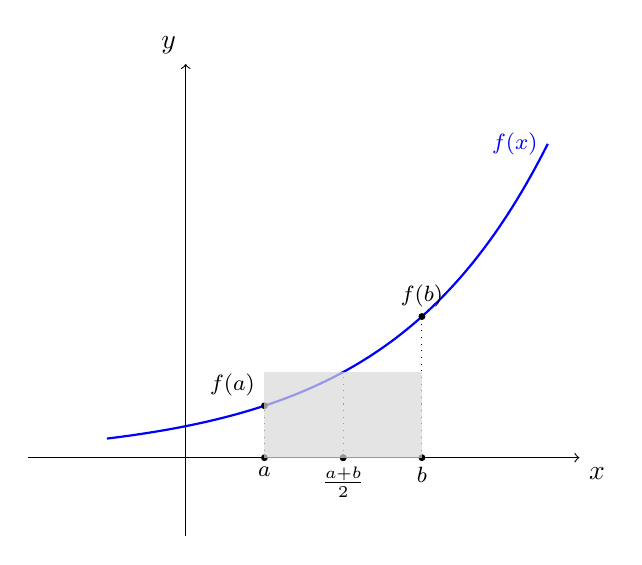
\begin{tikzpicture}[scale=2, domain=-0.5:2.3, samples=100]
	% draw axis
	\draw[->] (-1,0) -- (2.5,0) node[below right] {$x$};
	\draw[->] (0,-0.5) -- (0,2.5) node[above left] {$y$};
	
	% draw function
	\draw[blue, thick] plot (\x, {0.2*exp(\x)}) node[left] {\footnotesize $f(x)$};

	% draw x-axis intercept
    \def\x{0.5};
	\draw[dotted] (\x, 0) node[below] {\footnotesize $a$} -- (\x,{0.2*exp(\x)});
    \draw[fill=black] (\x,{0.2*exp(\x)}) circle [radius=0.018] node[above left] {\footnotesize $f(a)$};
    \draw[fill=black] (\x,0) circle [radius=0.018];
 
    \def\y{1.5};
	\draw[dotted] (\y, 0) node[below] {\footnotesize $b$} -- (\y,{0.2*exp(\y)});
	\draw[fill=black] (\y,0) circle [radius=0.018];
    \draw[fill=black] (\y,{0.2*exp(\y)}) circle [radius=0.018] node[above] {\footnotesize $f(b)$};

    \def\z{1};
    \draw[fill=black] (\z,0) circle [radius=0.018] node[below] {\footnotesize $\frac{a+b}{2}$};
    \draw[dotted] (\z, 0) -- (\z,{0.2*exp(\z)});
	\draw[fill=black] (\z,0) circle [radius=0.018];

    \fill[gray!30,opacity=0.7] (\x,0) rectangle (\y,{0.2*exp(\z)});
    \end{tikzpicture}$$
    Calculemos el error de esta fórmula. Sean $p_o$ y $p_1$ los polinomios de interpolación de $f$ en $\left\{\dfrac{a+b}{2}\right\}$ y $\left\{\dfrac{a+b}{2}\right\}$ respectivamente. Tenemos entonces que
    $$\mathcal{E}_o(f)=\int_a^b(f(x)-p_o(x))dx=\int_a^b(f(x)-p_1(x))dx=$$
    $$\dfrac{f''(\xi)}{2}\int_a^b\left(x-\dfrac{a+b}{2}\right)=\dfrac{f''(\xi)}{6}\left[\left(x-\dfrac{a+b}{2}\right)^3\right]_a^b=\dfrac{f''(\xi)}{24}(b-a)^3$$

\end{ejem}
\begin{ejem}(\textbf{Fórmula del trapecio})
Tomando $n=1$ en (\ref{form:int}) y  $x_o=a$ y $x_1=b$ se tiene que
$$\omega_o=\int_a^b \dfrac{x-b}{a-b}=\dfrac{1}{a-b}\cdot \left.\dfrac{(x-b)^2}{2}\right|_{a}^b=\dfrac{b-a}{2}$$
$$\omega_1=\int_a^b \dfrac{x-a}{b-a}=\dfrac{1}{b-a}\cdot \left.\dfrac{(x-a)^2}{2}\right|_{a}^b=\dfrac{b-a}{2}$$
y con lo cual
\begin{align}
\int_a^bf(x)dx\approx\dfrac{b-a}{2}(f(a)+f(b))
\label{trapecio}    
\end{align}
Podemos visualizar esta aproximación de la siguiente forma
$$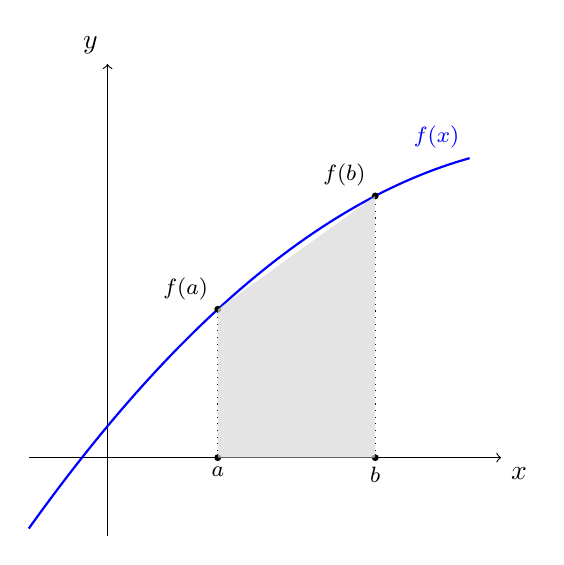
\begin{tikzpicture}[scale=2, domain=-0.5:2.3, samples=100]
	
	% draw axis
	\draw[->] (-0.5,0) -- (2.5,0) node[below right] {$x$};
	\draw[->] (0,-0.5) -- (0,2.5) node[above left] {$y$};
	
	% draw function
	\draw[blue, thick] plot (\x, {-0.2*(\x-3)*(\x-3)+2}) node[above left] {\footnotesize $f(x)$};

	% draw x-axis intercept
    \def\x{0.7};
	\draw[dotted] (\x, 0) node[below] {\footnotesize $a$} -- (\x,{-0.2*(\x-3)*(\x-3)+2});
    \draw[fill=black] (\x,{-0.2*(\x-3)*(\x-3)+2}) circle [radius=0.018] node[above left] {\footnotesize $f(a)$};
    \draw[fill=black] (\x,0) circle [radius=0.018];
 
    \def\y{1.7};
	\draw[dotted] (\y, 0) node[below] {\footnotesize $b$} -- (\y,{-0.2*(\y-3)*(\y-3)+2});
	\draw[fill=black] (\y,0) circle [radius=0.018];
    \draw[fill=black] (\y,{-0.2*(\y-3)*(\y-3)+2}) circle [radius=0.018] node[above left] {\footnotesize $f(b)$};

    \fill[gray!30,opacity=0.7] (\x,0) -- (\y,0) -- (\y,{-0.2*(\y-3)*(\y-3)+2}) -- (\x,{-0.2*(\x-3)*(\x-3)+2});
	
    \end{tikzpicture}$$
     Calculemos a continuación el error. Tomando $n=1$ en (\ref{error:integ} obtenemos lo siguiente:
     $$\mathcal{E}_1(f)=\dfrac{f''(\xi)}{2}\int_a^b(x-a)(x-b)$$
     Realizamos el siguiente cambio de variable
     $$x=\dfrac{a+b}{2}+t\dfrac{b-a}{2}$$
     $$dx=\dfrac{b-a}{2}t$$
     Teniéndose entonces que
     $$\mathcal{E}_1(f)=\dfrac{f''(\xi)}{2}\cdot \dfrac{b-a}{2}\int_{-1}^1\left(\dfrac{a+b}{2}+t\dfrac{b-a}{2}-a\right)\left(\dfrac{a+b}{2}+t\dfrac{b-a}{2}-b\right)dx=$$
     $$\dfrac{f''(\xi)}{2}\cdot \left(\dfrac{b-a}{2}\right)^3\int_{-1}^1(t^2-1)dt=-\dfrac{f''(\xi)}{12}(b-a)^3$$
\end{ejem}
\begin{ejem}
(\textbf{Fórmula de Simpson})
Estudiemos el caso $n=2$. Si denotamos por $p_1(x)$ al polinomio de interpolación de $f$ en $\{a,b\}$ y por $p_2(x)$ al polinomio de interpolación en los nodos $\left\{a,\dfrac{a+b}{2},b\right\}$ sabemos por (\ref{ec:newton}) que
$$\int_a^bp_2(x)=\int_a^bp_1(x)+f\left[a,\dfrac{a+b}{2},b\right]\cdot \int_a^b(x-a)(x-b)dx$$
Integrando por partes y aplicando la fórmula del trapecio tenemos que
$$\int_a^bp_2(x)=\dfrac{b-a}{2}(f(a)+f(b))+\frac{\Delta^2f(a)}{2\left(\dfrac{b-a}{2}\right)^2}\cdot \left((x-a)\dfrac{(x-b)^2}{2}-\dfrac{(x-b)^3}{6}dx\right)_a^b=$$
$$=\dfrac{b-a}{2}(f(a)-f(b))-\dfrac{2f(a)-4f\left(\dfrac{a+b}{2}\right)+2f(b)}{(b-a)^2}\cdot \dfrac{(b-a)^3}{6}=$$
$$=\dfrac{b-a}{6}(f(a)+4f\left(\dfrac{a+b}{2}\right)+f(b))$$
Deduciendo entonces la fórmula:
\begin{align}
 \int_a^{b}f(x)dx\approx \dfrac{b-a}{6}(f(a)+4f\left(\dfrac{a+b}{2}\right)+f(b))
 \label{simpson}
\end{align}
%$$\begin{tikzpicture}[scale=2, domain=-0.5:2, samples=100]
	% draw axis
%	\draw[->] (-0.5,0) -- (2.5,0) node[below right] {$x$};
%	\draw[->] (0,-0.5) -- (0,2.5) node[above left] {$y$};
	
	% draw function
%	\draw[blue, thick] plot (\x,{2*cos(\x r)}) node[above left] {\footnotesize $f(x)$};
	% draw x-axis intercept
  %  \def\x{0.2};
%	\draw[dotted] (\x, 0) node[below] {\footnotesize $a$} -- (\x,{2*cos(\x r)});
%    \draw[fill=black] (\x,{2*cos(\x r)}) circle [radius=0.018] node[above right] {\footnotesize $f(a)$};
 %   \draw[fill=black] (\x,0) circle [radius=0.018];
 
  %  \def\y{1.45};
%	\draw[dotted] (\y, 0) node[below] {\footnotesize $b$} -- (\y,{2*cos(\y r)});
%	\draw[fill=black] (\y,0) circle [radius=0.018];
 %   \draw[fill=black] (\y,{2*cos(\y r)}) circle [radius=0.018] node[above right] {\footnotesize $f(b)$};

 %   \def\z{0.825};
%	\draw[dotted] (\z, 0) node[below] {\footnotesize $\dfrac{a+b}{2}$} -- (\z,{2*cos(\z r)});
%	\draw[fill=black] (\z,0) circle [radius=0.018];

%	\fill[gray!30,opacity=0.7] (\x,0) -- (\y,0) -- (\y,{1.02237-0.145829*\y-0.328377*\y*\y}) -- (\x,{1.02237-0.145829*\x-0.328377*\x*\x});%
%	
Veamos ahora el error de la fórmula obtenida. Sean $p_2(x)$ y $p_3(x)$ los polinomios de interpolación de $f(x)$ en $\left\{a,\dfrac{a+b}{2},b\right\}$ y $\left\{a,\dfrac{a+b}{2},\dfrac{a+b}{2},b\right\}$. Se tiene entonces que
$$\mathcal{E}_2(f)=\int_a^b(f(x)-p_2(x))dx=\int_a^b(f(x)-p_3(x))dx=\dfrac{f^{(4)}(\xi)}{4!}\int_a^b(x-a)\left(x-\dfrac{a+b}{2}\right)^2(x-b)dx$$
Volviendo a realizar el cambio de variable $x=\dfrac{a+b}{2}+t\dfrac{b-a}{2}$ concluimos lo siguiente:
$$\mathcal{E}_2(f)=\dfrac{f^{(4)}(\xi)}{4!}\cdot \left(\dfrac{b-a}{2}\right)^5\int_{-1}^1t^2(t^2-1)dx=-\dfrac{f^{(4)}(\xi)}{90}\cdot \left(\dfrac{b-a}{2}\right)^5$$

\end{ejem}
\begin{obs}
Llamaremos \textbf{fórmulas de Newton-Côtes} a las fórmulas de cuadratura de tipo interpolatorio para un conjunto de nodos equidistantes. Si tomamos $h=\dfrac{b-a}{2}$ podemos expresar la fórmula de Simpson en la forma ''un tercio'':
$$\int_a^{b}f(x)dx\approx \dfrac{h}{3}(f(a)+4f\left(a+h\right)+f(a+2h))$$
\end{obs}

 \section{Fórmulas compuestas}

 \begin{obs}
Se trata de calcular la integral buscada por una suma de integrales aproximadas, esto es
$$\int_a^bf(x)=\sum_{i=0}^n\int_{x_i}^{x_{i+1}}f(x)dx$$
donde $x_i=a+i\cdot \dfrac{b-a}{n}$. 
 \end{obs}
 \begin{ejem}[\textbf{Fórmula del trapecio compuesto}] Aproximaremos cada una de las integrales del sumatorio anterior por la fórmula del trapecio:
$$\int_a^bf(x)=\sum_{i=0}^{n-1}\int_{x_i}^{x_{i+1}}f(x)dx\approx\sum_{i=0}^{n-1}\left(\dfrac{x_{i+1}-x_i}{2}\cdot(f(x_i)+f(x_{i+1}))\right)$$
tomando ahora $h_n=\dfrac{b-a}{n}$ se tiene que
 $$\int_a^bf(x)dx\approx\dfrac{h_n}{2}\sum_{i=0}^{n-1}(f(x_i)+f(x_{i+1}))=$$
 \begin{align}
  =\dfrac{h_n}{2}\left(f(a)+2\sum_{i=1}^{n-1}f(x_i)+f(b)\right)
  \label{trp:comp}
 \end{align}
 Para calcular el error de esta fórmula sumaremos los errores en cada uno de los intervalos, esto es:
 $$\mathcal{E}_{TC}(f)=\sum_{i=0}^{n-1}-\dfrac{f''(\xi_i)}{12}\left(\dfrac{b-a}{n}\right)^3=-\dfrac{f''(\xi)}{12}\left(\dfrac{b-a}{n}\right)^3\cdot n=$$
 $$=-\dfrac{f''(\xi)}{12}(b-a)h_n^2$$
 Donde hemos usado que si $f $ es continua se verifica que
 $$\sum_{i=1}^nc_i\cdot f(x_i)=f(\xi)\cdot \sum_{i=1}^nc_i$$
 \end{ejem}

 \begin{ejem}
    (\textbf{Fórmula de Simpson compuesta}) Si utilizamos la fórmula de Simpson para aproximar las integrales del sumatorio inicial obtenemos lo siguiente:
    $$\int_a^bf(x)dx\approx\sum_{i=0}^{n-1}\left(\dfrac{x_{i+1}-x_i}{6}(f(x_i)+4f\left(\dfrac{x_i+x_{i-1}}{2}\right)+f(x_{i+1}))\right)$$
    Tomando ahora $h_n=\dfrac{b-a}{2n}$ tenemos que
    $$\int_a^bf(x)dx\approx\dfrac{h_n}{3}\sum_{i=0}^{n-1}(f(x_i)+4f\left(\dfrac{x_i+x_{i-1}}{2}\right)+f(x_{i+1}))=$$
    \begin{align}
    =\dfrac{h_n}{3}\left(f(a)+2\sum_{i=1}^{n-1}f(x_i)+4\sum_{i=0}^{n-1}f\left(\dfrac{x_i+x_{i-1}}{2}\right)+f(b)\right)
    \label{simp:comp}     
    \end{align}
    Calcularemos el error de esta fórmula como antes, sumando el arror en cada uno de los intervalos:
    $$\mathcal{E}_S(f)=\sum_{i=0}^{n-1}-\dfrac{f^{(4)}(\xi_i)}{90}\left(\dfrac{b-a}{2n}\right)^5=-\dfrac{f^{(4)}(\xi)}{90}\left(\dfrac{b-a}{2n}\right)^5\cdot n=$$
    $$=-\dfrac{f^{(4)}(\xi)}{180}(b-a)h_n^4$$
 \end{ejem}
  \begin{ejem}
Aproximaremos la integral $\int_o^{\frac{\pi}{2}}\cos x dx$ con las fórmulas del trapecio y de Simpson compuestas. Dividiendo el intervalo en 2 partes ($n=2$) obtenemos la siguiente aproximación pra la fórmula del trapecio
 $$\int_0^{\frac{\pi}{2}}\cos (x) dx\approx \dfrac{\pi}{8}(\cos(o)+2\cos\left(\dfrac{\pi}{4}\right)+\cos\left(\dfrac{\pi}{2}\right)\approx 0.948$$
 Hemos obtenido una precisión bastante aceptable (el valor real de la integral es $1$). Utilizando ahora la fórmula de Simpson compuesta para $n=2$:
 $$\int_0^{\dfrac{\pi}{2}}\cos x dx\approx\dfrac{\pi}{24}(\cos(0)+4\cos\left(\dfrac{\pi}{8}\right)+2\cos\left(\dfrac{\pi}{4}\right)+4\cos\left(\dfrac{\pi}{4}\right)+4\cos\left(\dfrac{3\pi}{8}\right)+\cos\left(\dfrac{\pi}{2}\right)\approx1.0001$$
 \end{ejem}

 \section{Cuadraturas adaptativas}
\begin{met}(\textbf{de las cuadraturas adaptativas})
Queremos aproximar la integral $\int_a^bf(x)dx$ con una tolerancia $\varepsilon$. Supongamos que tenemos una fórmula de cuadratura $I(f)$ para aproximar dicha integral con una tolerancia superior a la requerida. Dividiremos entonces el intervalo el intervalo $[a,b]$ en subintervalos más pequeños $[x_{-1},x_{i}]$ de longitud variable y aproximaremos cada una de las integrales por la fórmula $I(f)$:
$$\int_a^bf(x)dx=\sum_{i=1}^n(I_i(f)+e_i)=\sum_{i=1}^nI_i(f)+\sum_{i=1}^ne_i$$
Donde $I_{i}(f)+e_i=\int_{x_{i-1}}^{x_i}f(x)dx$, siendo $e_i$ el error local. Observemos entonces que si
$$|e_i|\leq\varepsilon\cdot\dfrac{x_i-x_{i-1}}{b-a}$$
Entonces el error total estará acotado por
$$\left|\sum_{i=1}^ne_i\right|\leq\sum_{i=1}^n|e_i|\leq\dfrac{\varepsilon}{b-a}\sum_{i=1}^n(x_{i}-x_{i-1})=\varepsilon$$
Esto nos da una condición para determinar si es necesario dividir el intervalo $[x_{i-1},x_i]$, esto es, si la fórmula $I_i(f)$ tiene un error superior a la cantidad $\varepsilon\cdot\dfrac{x_i-x_{i-1}}{b-a}$ tendremos que dividir el intervalo y, en caso contrario, no será necesario.


\end{met}
 \begin{ejem}
    (\textbf{Fórmula del trapecio adaptativa}) Si aproximamos $\int_a^bf(x)dx$ por la fórmula del trapecio tenemos que
    $$\int_a^bf(x)dx=\dfrac{b-a}{2}(f(a)-f(b))-\dfrac{f''(\xi)}{12}(b-a)^3=T-\dfrac{f''(\xi)}{12}(b-a)^3$$
    Si dividimos el intervalo $[a,b]$ en dos:
    $$\int_a^bf(x)dx=\int_a^{\frac{a+b}{2}}f(x)dx+\int_{\frac{a+b}{2}}^bf(x)dx=T_1+T_2-\dfrac{f''(\xi_1)}{12}\left(\dfrac{b-a}{2}\right)^3-\dfrac{f''(\xi_2)}{12}\left(\dfrac{b-a}{2}\right)^3$$
    Y por el Teorema del Valor Medio sabemos que existe $\bar{\xi}\in[a,b]$ tal que $f''(\bar{\xi})=\frac{f''(\xi_1)+f''(\xi_2)}{2}$, con lo cual
    $$\int_a^bf(x)dx=T_1+T_2-\dfrac{f''(\bar{\xi})}{12}\cdot \dfrac{(b-a)^3}{4}$$
    Sea $h=b-a$, si suponemos entonces que $f''(\bar{\xi})\approx f''(\xi)$, podemos aproximar el error de la fórmula anterior de la siguiente forma:
    $$\int_a^bf(x)dx=T-\dfrac{f''(\bar{\xi})}{12}\cdot h^3= T_1+T_2-\dfrac{f''(\bar{\xi})}{12}\cdot \dfrac{h^3}{4}$$
    $$T-(T_1+T_2)\approx-\dfrac{f''(\bar{\xi})}{12}\cdot \dfrac{h^3}{4}\cdot (-3)$$
    De manera que
    $$\dfrac{-1}{3}(T-(T_1+T_2))\approx -\dfrac{f''(\xi)}{12}\cdot \dfrac{h^3}{4}$$
    Si el error es menor que la tolerancia esperada $\varepsilon$ aceptamos el trapecio compuesto como valor para la integral:
    \begin{align}
     \int_a^bf(x)dx\approx T_1+T_2-\dfrac{1}{3}(T-(T_1+T_2))
     \label{trap:adap}
    \end{align}
    Con lo cual, si se verifica que
    $$\dfrac{1}{3}|T-(T_1+T_2)|<\varepsilon$$
    tomaremos la aproximación como válida. En caso contrario, debemos dividir el intervalo en más subvintervalos. Consideremos por ejemplo el intervalo de la derecha $\left[\dfrac{a+b}{2},b\right]$ y apliquemos el mismo razonamiento:
    $$\int_{\frac{a+b}{2}}^bf(x)dx=T_{21}+T_{22}-\dfrac{1}{3}(T_2-(T_{21}+T_{22})$$
    Y por tanto, si se verifica que
    $$\dfrac{1}{3}|T_2-(T_{21}+T_{22})|<\dfrac{\varepsilon}{2}$$
    tomaremos la aproximación como válida y, en caso contrario, reiteraríamos el mismo proceso hasta obtener la precisión requerida. 
 \end{ejem}
 \begin{ejer}
    Aproximar la integral $\int_0^{\frac{\pi}{2}}cos(x)dx$ por la fórmula del trapecio adaptativa con error menor que $\varepsilon=10^{-2}$.
 \end{ejer}
 \begin{sol}
Con las notaciones precedentes tenemos que
$$T=\dfrac{\pi}{4}(\cos(0)+\cos\left(\dfrac{\pi}{2}\right))\approx 0.785398$$
$$T_1=\dfrac{\pi}{8}(\cos(0)+\cos\left(\dfrac{\pi}{4}\right))\approx 0.670379$$
$$T_2=\dfrac{\pi}{8}(\cos\left(\dfrac{\pi}{4}\right)+\cos\left(\dfrac{\pi}{2}\right))\approx 0.277680$$
Y por tanto
$$\dfrac{1}{3}|T-(T_1+T_2)|\approx 0.054>\varepsilon$$
Luego la aproximación no es lo suficientemente buena y por tanto tenemos que dividir el intervalo en más subintervalos. Dividamos en primer lugar elintervalo más a la derecha $\left[\dfrac{\pi}{4},\dfrac{\pi}{2}\right]$:
$$T_2=0.277680$$
$$T_{21}=\dfrac{\pi}{16}(\cos\left(\dfrac{\pi}{4}\right)+\cos\left(\dfrac{\pi}{4}+\dfrac{\pi}{8}\right))\approx 0.213980$$
$$T_{22}=\dfrac{\pi}{16}(\cos\left(\dfrac{3\pi}{8}\right)+\cos\left(\dfrac{\pi}{2}\right)\approx 0.075140$$
Con lo cual
$$\dfrac{1}{3}|T_2-(T_{12}+T_{22})|\approx 0.0038<\dfrac{\varepsilon}{2}$$
Y tomamos como aceptable la aproximación. Trabajemos ahora en el intervalo $\left[0,\dfrac{\pi}{4}\right]$:
$$T_1=0.670379$$
$$T_{11}=\dfrac{\pi}{16}(\cos(0)+\cos\left(\dfrac{\pi}{8}\right))=0.377753$$
$$T_{12}=\dfrac{\pi}{16}(\cos\left(\dfrac{\pi}{8}\right)+\cos\left(\dfrac{\pi}{4}\right))=0.320243$$
Veamos entonces si la aproximación es válida:
$$|T_1-(T_{11}+T_{12})|\approx 9\cdot 10^{-3}>\dfrac{1}{2}\varepsilon$$
Luego debemos seguir dividiendo este intervalo a la mitad. Consideremos entonces el intervalo $\left[\dfrac{\pi}{8},\dfrac{\pi}{4}\right]$:
$$T_{12}=0.320243$$
$$T_{121}=\dfrac{\pi}{32}(\cos\left(\dfrac{\pi}{8}\right)+\cos\left(\dfrac{\pi}{8}+\dfrac{\pi}{16}\right))\approx0.172331$$
$$T_{122}=\dfrac{\pi}{32}(\cos\left(\dfrac{3\pi}{16}\right)+\cos\left(\dfrac{\pi}{4}\right))\approx0.151049$$
El error cometido será:
$$|T_{12}-(T_{121}+T_{122})|\approx 0.001<\dfrac{1}{4}\varepsilon$$
Luego aceptamos la aproximación. Estudiemos entonces el intervalo que falta $\left[0,\dfrac{\pi}{8}\right]$:
$$T_{11}=0.377753$$
$$T_{111}=\dfrac{\pi}{32}(\cos(0)+\cos\left(\dfrac{\pi}{16}\right))\approx0.194463$$
$$T_{112}=\dfrac{\pi}{32}(\cos\left(\dfrac{\pi}{16}\right)+\cos\left(\dfrac{\pi}{8}\right))\approx 0.186990$$
Teniendose entonces un error de
$$|T_{11}-(T_{111}+T_{112})|\approx 0.00.<\dfrac{1}{4}\varepsilon$$
En conclusión, el valor de la integral obtenido es
$$\int_0^{\frac{\pi}{2}}cos(x)dx\approx0.292933+0.324426+0.382686=1.00005$$
Como el valor de la integral es exactamente $1$, el error cometido es mínimo .

 \end{sol}
 \newpage
 \begin{ejem}
     (\textbf{Fórmula de Simpson adaptativa})
     Si aproximamos $\int_a^bf(x)dx$ por la fórmula de Simpson tenemos que
   $$\int_a^{b}f(x)dx= \dfrac{b-a}{6}(f(a)+4f\left(\dfrac{a+b}{2}\right)+f(b))-\dfrac{f^{(4)}(\xi)}{90}\left(\dfrac{b-a}{2}\right)^5=S-\dfrac{f^{(4)}(\xi)}{90}\left(\dfrac{b-a}{2}\right)^5$$
    Si dividimos el intervalo $[a,b]$ en dos:
    $$\int_a^bf(x)dx=\int_a^{\frac{a+b}{2}}f(x)dx+\int_{\frac{a+b}{2}}^bf(x)dx=S_1+S_2-\dfrac{f^{(4)}(\xi_1)}{90}\left(\dfrac{b-a}{4}\right)^5-\dfrac{f^{(4)}(\xi_2)}{90}\left(\dfrac{b-a}{4}\right)^5$$
    Y por el teorema del valor intermedio sabemos que existe $\bar{\xi}\in[a,b]$ tal que $f^{(4)}(\bar{\xi})=\frac{f^{(4)}(\xi_1)+f^{(4)}(\xi_2)}{2}$, con lo cual
    $$\int_a^bf(x)dx=S_1+S_2-\dfrac{f^{(4)}(\bar{\xi})}{1440}\cdot \left(\dfrac{b-a}{2}\right)^5$$
    Sea $h=\frac{b-a}{2}$, si suponemos entonces que $f^{(4)}(\bar{\xi})\approx f^{(4)}(\xi)$, podemos aproximar el error de la fórmula anterior de la siguiente forma:
    $$\int_a^bf(x)dx=S-\dfrac{f^{(4)}(\xi)}{90}\cdot h^5= S_1+S_2-\dfrac{f^{(4)}(\bar{\xi})}{1440}\cdot h^5$$
    $$S_1+S_2-S\approx\dfrac{-5f^{(4)}(\xi)}{480}h^5$$
    De manera que
    $$\dfrac{1}{15}(S_1+S_2-S)\approx -\dfrac{f^{(4)}(\xi)}{1440}h^5$$
    Si el error es menor que la tolerancia esperada $\varepsilon$ aceptamos el trapecio compuesto como valor para la integral:
    \begin{align}
    \int_a^bf(x)dx\approx S_1+S_2+\dfrac{1}{15}(S_1+S_2-S)
    \label{simp:adap}
    \end{align}
    Con lo cual, si se verifica que
    $$\dfrac{1}{15}|S_1+S_2-S|<\varepsilon$$
    tomaremos la aproximación como válida. En caso contrario, debemos dividir el intervalo en más subvintervalos. Consideremos por ejemplo el intervalo de la derecha $\left[\dfrac{a+b}{2},b\right]$ y apliquemos el mismo razonamiento:
    $$\int_{\frac{a+b}{2}}^bf(x)dx=S_{21}+S_{22}+\dfrac{1}{15}(S_1+S_2-S)$$
    Y por tanto, si se verifica que
    $$\dfrac{1}{15}|S_{21}+S_{22}-S_2|<\dfrac{\varepsilon}{2}$$
    tomaremos la aproximación como válida y, en caso contrario, reiteraríamos el mismo proceso hasta obtener la precisión requerida. 
 \end{ejem}
\section{Cuadraturas gaussianas}
\begin{defin} Las \textbf{cuadraturas gaussianas} son fórmulas para aproximar integrales del tipo $\displaystyle \int_a^b f(x)\cdot \omega(x)dx$, siendo $\omega(x)$ una función peso
$$\int_a^b f(x)\cdot \omega(x)dx\approx\sum_{i=1}^n\omega_if(x_i)$$
que son exactas para polinomios de grado menor o igual que $2n-1$.   
\end{defin}                            
\begin{ejem}
 Para $n=1$ y $\omega(x)$=1, tendremos que la fórmula es exacta para polinomios de grado menor o igual que 1. Tomando la base $\{1,x\}$ en $\mathbb{P}_1[x]$ calculamos $x_1$ y $\omega_1$:
 $$\int_a^bdx=b-a=\omega_1$$
 $$\int_a^bxdx=\dfrac{b^2-a^2}{2}=\dfrac{(b-a)(b+a)}{2}=\omega_1x_1\Longrightarrow x_1=\dfrac{b+a}{2}$$
 Y la fórmula obtenida es la del punto medio:
 $$\int_a^bf(x)dx\approx(b-a)\cdot f\left(\dfrac{b+a}{2}\right)$$
\end{ejem}
\begin{ejem}
Fijemos el intervalo de referencia $[-1,1]$. Para $n=2$ y $\omega(x)=1$ la fórmula será exacta para los polinomios de $\mathbb{P}_3[x]$, luego tomemos la base $\{1,x,x^2,x^3\}$:
$$\int_1^{-1}dx=2=\omega_1+\omega_2$$
$$\int_1^{-1}xdx=0=\omega_1x_1+\omega_2x_2$$
$$\int_1^{-1}x^2dx=\dfrac{2}{3}=\omega_1x_1^2+\omega_2x_2^2$$
$$\int_1^{-1}x^3dx=0=\omega_1x_1^3+\omega_2x_2^3$$
De la segunda ecuación deducimos que $\omega_1x_1=-\omega_2x_2$, con lo cual:
$$0=\omega_1x_1^3+\omega_2x_2^3=\omega_1x_1(x_1^2-x_2^2)\Rightarrow x_1^2=x_2^2$$
Y por ser $x_1\neq x_2$ tenemos que $x_1=-x_2$. Utilizando esto en la segunda acuación $\omega_1=\omega_2$ y, por la primera ecuación, concluimos que $\omega_1=1$. Podemos despejar $x_1$ de la tercera ecuación:
$$\dfrac{2}{3}=2\omega_1 x_1\Rightarrow x_1=\dfrac{1}{\sqrt{3}}$$
La fórmula obtenida será, por tanto
$$\int_{-1}^1f(x)\approx f\left(\dfrac{1}{\sqrt{3}}\right)+f\left(-\dfrac{1}{\sqrt{3}}\right)$$
que denominaremos más adelante como fórmula de Gauss-Legendre de dos puntos.
\end{ejem}

\subsection{Cálculo de los nodos}
\begin{defin}
Definimos en $\mathbb{P}_n[x]$ el siguiente producto escalar:
$$g_{\omega}(p,q)=\int_a^b p(x) \cdot q(x)\cdot \omega(x) \: dx$$
 con $\omega(x)>0\;\forall x\in[a,b]$.
\end{defin}
\begin{obs}
Construiremos a continuación una base  $\{p_o,p_1,\ldots,p_n\}$ de polinomios mónicos ortogonales con respecto a la métrica $g_{\omega}$ utilizando técnicas similares a la ortonormalización de Gram-Schmidt. Esto es, que para cualquier polinomio $q_k(x)$ de grado $k\leq n-1$ 
$$\int_a^bp_n(x)\cdot q_k(x)\omega(x)dx=0$$
\end{obs}
\begin{prop}
Con las notaciones precedentes, se tiene que
$$p_o=1$$
$$p_1=x-\dfrac{g_{\omega}(x,1)}{g_{\omega}(1,1)}$$
\begin{align}
 p_{n+1}=\left(x-\alpha_{n+1}\right)\cdot p_n- \gamma_{n+1}^2\cdot p_{n-1}
 \label{pol:gauss}
\end{align}
donde
$$\alpha_{n+1}=\dfrac{g_{\omega}(p_n,xp_n)}{g_{\omega}(p_{n},p_{n})}\qquad \gamma_{n+1}^2=\dfrac{g_{\omega}(p_n,p_n)}{g_{\omega}(p_{n-1},p_{n-1})}$$
\end{prop}
\begin{dem}
Construyamos los polinomios $p_n(x)$. Definimos primero $p_o=1$ y sea \newline $p_1=x+\alpha_1$. Determinamos $\alpha_1$ por la condición de ortogonalidad:
$$0=g_{\omega}(p_o,p_1)=\int_a^b(x+\alpha_1)\omega(x)=\int_a^bx\omega(x)dx+\alpha_1\int_a^b\omega(x)dx$$
$$\alpha_1=-\dfrac{g_{\omega}(x,1)}{g_{\omega}(1,1)}$$
Supongamos entonces que tenemos construidos $\{p_o,p_1,\ldots,p_n\}$ y construyamos $p_{n+1}$. Por ser una base de polinomios mónicos, sabemos que $p_{n+1}-xp_n$ es de grado $n$, luego se puede expresar como combinación lineal de los elementos de la base:
$$p_{n+1}-xp_n=\delta_{n+1}p_n+\sum_{j=0}^{n-1}\beta_jp_j$$
y con lo cual
$$p_{n+1}=(x+\delta_{n+1})p_n+\sum_{j=0}^{n-1}\beta_jp_j$$
Los coeficientes $\alpha_{n+1},\beta_j$ se calculan imponiendo las condiciones de ortogonalidad.
$$g_{\omega}(p_{n+1},p_i)=0\qquad i=0,\ldots,n$$
Operando se tiene que
$$0=g_{\omega}(p_{n+1},p_i)=g_{\omega}(xp_n,p_i)+\delta_{n+1}g_{\omega}(p_n,p_i)+\sum_{j=0}^{n-1}\beta_jg_{\omega}(p_j,p_i)$$
Por la definición de $g_{\omega}$, sabemos que $g_{\omega}(xp_n,p_i)=g_{\omega}(p_n,xp_i)$. Por tanto, si $i<n-1$ sabemos que $p_n$ es ortogonal a $p_i$ y al multiplicarlo por $x$ obtendremos un polinomio de grado estrictamente menor que $n$, luego $p_n$ seguirá siendo ortogonal a dicho polinomio. Con esto podemos concluir que los dos primeros términos son nulos. Además, como $p_j$ es ortogonal a $p_i$, tenemos que
$$0=\sum_{j=0}^{n-1}\beta_jg_{\omega}(p_j,p_i)=\beta_ig_{\omega}(p_i,p_i)\Rightarrow \beta_i=0$$
Para $i=n-1$ sabemos que$g_{\omega}(p_j,p_{n-1})=0,\, \forall j<n-1$ con lo cual
$$0=g_{\omega}(p_{n+1},p_{n-1})=g_\omega(xp_n,p_{n-1})+\delta_{n+1}g_{\omega}(p_n,p_{n-1})+\beta_{n-1}g_{\omega}(p_{n-1},p_{n-1})=$$
$$=g_{\omega}(p_n,xp_{n-1})+\beta_{n-1}g_{\omega}(p_{n-1}p_n-1)\Rightarrow\beta_{n-1}=-\dfrac{g_{\omega}(p_n,p_n)}{g_{\omega}(p_{n-1},p_{n-1}}$$
donde hemos empleado que
$$g_{\omega}(p_{n},p_{n-1})=g_{\omega}(p_n,p_n+xp_{n-1}-p_n)=g_{\omega}(p_n,p_n)+g_{\omega}(p_n,xp_{n-1}-p_n)=g_{\omega}(p_n,p_n)$$
ya que $xp_{n-1}-p_n$ es de grado $n-1$. 
Tomando ahora $i=n$ 
$$0=g_{\omega}(p_{n+1},p_n)=g_{\omega}(p_n,xp_n)+\alpha_{n+1}g_{\omega}(p_n,p_n)$$
y despejando
$$\alpha_{n+1}=-\dfrac{g_{\omega}(p_n,xp_n)}{g_{\omega}(p_n,p_n)}$$
    
\qed\end{dem}

 \begin{prop}
Con las notaciones precedentes, las raíces de $p_n$ son reales, simples y están en $[a,b]$
 \end{prop}
 \begin{dem}
 La raíces de $p_n(x)$ se clasifican en cuatro conjuntos disjuntos: \vspace{-5mm}
 \begin{itemize}
 \item[a)] Raíces complejas
 \item[b)] Raíces reales fuera del intervalo $[a,b]$
 \item[c)] Raíces reales dentro del intervalo $[a,b]$ de multiplicidad par
 \item[d)] Raíces reales dentro del intervalo $[a,b]$ de multiplicidad impar
 \end{itemize}
 Sean $x_1,\ldots,x_s$ las raíces reales de $p_n$ dentro del intervalo $[a,b]$ de multiplicidad impar y sea $q_s=\prod_{i=1}^s(x-x_s)$.
 
 Con lo cual, los puntos $x_1,\ldots,x_s$ serán raíces de multiplicidad par del polinomio $p_{n}\cdot q_s$. Por tanto, solo tendrá raíces complejas, de multiplicidad par o fuera del intervalo, luego el polinomio $p_{n}\cdot q_s$ no cambia de signo en el intervalo $[a,b]$, con lo cual:
 $$g_{\omega}(p_n,q_s)=\int_{a}^bp_n(x)q_s(x)\omega(x)dx\neq 0$$
 Como $p_n$ es ortogonal a todos los polinomios de grado menor que $n$, la única opción es que $s=n$ y, por tanto, todas las raíces de $p_n$ son reales, están en el intervalo $[a,b]$ y tienen multiplicidad $1$.
 
 \qed\end{dem}
 \begin{defin}
    Diremos que las funciones $\{\phi_1,\ldots,\phi_n\}$ satisfacen la \textbf{condición de Haar} cuando
    $$\left|\begin{array}{ccc}
      \phi_1(t_1)&\cdots   &\phi_n(t_1)  \\
        \vdots &\ddots&\vdots \\
         \phi_1(t_n)&\cdots   &\phi_n(t_n)
    \end{array}\right|\neq 0$$
    para cualesquiera $t_1,\ldots,t_n$ distintos entre sí.
 \end{defin}
 \begin{prop}
Los polinomios $\{p_o,\ldots,p_n\}$ satisfacen la condición de Haar.
 \end{prop}
 \begin{dem}
Si $t_o,\ldots,t_n$ son $n+1$ puntos distintos, las formas lineales $\sigma_i(p(x))=p(t_i)$ son linealmente independientes y, por tanto, base de $\mathbb{P}_{n}^*[x]$. Además, sabemos que los polib¡nomios $\{p_o,\ldots,p_n\}$ son base de $\mathbb{P}_n[x]$ (por ser ortogonales). Por último, obsrvemos que la matriz
$$\left(\begin{array}{ccc}
      p_o(t_o)&\cdots   &p_n(t_o)  \\
        \vdots &\ddots&\vdots \\
         p_o(t_n)&\cdots   &p_n(t_n)
    \end{array}\right)$$
    es la matriz de cambio de base de $\{p_o,\ldots,p_n\}$ a la base $\{\ell_o,\ldots,\ell_n\}$ (base dual de las $\sigma_i$), con lo que acabamos (por ser isomorfismo).
 \qed\end{dem}
 \begin{teo}
\item[a)]Sean $x_1,\ldots,x_n$ las raíces del polinomio ortogonal $p_n(x)$ y $\omega_1,\ldots,\omega_n$ las soluciones del sistema
$$\sum_{i=1}^n\omega_i\cdot p_j(x_i)=\left\{\begin{array}{cc}
   g_{\omega}(p_o,p_o)  & j=0  \\
    0 & j=1,\ldots,n
\end{array}\right.$$
Entonces la cuadratura 
$$\int_a^bf(x)dx\approx\sum_{i=1}^n\omega_if(x_i)$$
es exacta para los polinomios de grado menor o igual que $2n-1$ y $\omega_i>0$.
\item[b)] Recíprocamente, si  
$$\int_a^bf(x)dx\approx\sum_{i=1}^n\omega_if(x_i)$$
es una fórmula de cuadratura exacta para los polinomios de grado menor o igual que $2n-1$, entonces $x_1,\ldots,x_n$ son las raíces de $p_n(x)$ y los pesos $\omega_i$ son las soluciones del sistema enunciado.
\item[c)] No existe ninguna cuadratura de la forma 
$$\int_a^bf(x)dx\approx\sum_{i=1}^n\omega_if(x_i)$$
que sea exacta para todos los polinomios de grado $2n$.
 \end{teo}
 \begin{dem}
    \item[a)] Veamos entonces que la cuadratura es exacta para los polinomios de grado menor o igual que $2n-1$. Dado $q_m(x)$ de grado $m\leq 2n-1$, lo dividimos por $p_n(x)$
    $$q_m(x)=c(x)\cdot p_n(x)+r(x)$$
    de manera que
    $$\int_a^b q_m(x)\omega(x)dx=g_{\omega}(q_m,p_o)=g_{\omega}(c,p_n)+g_{\omega}(r,p_o)$$
    Como el grado de $c(x)$ es menor que el de $p_n(x)$, el primer término es nulo. Por otro lado, como $r(x)$ es de grado menor o igual que $n-1$ lo podemos expresar como $r(x)=\sum_{j=0}^{n-1}\beta_jp_j(x)$, de forma que
    $$\int_a^b q_m(x)\omega(x)dx=\sum_{j=0}^{n-1}\beta_j g_{\omega}(p_j,p_o)=\beta_o g_{\omega}(p_o,p_o)$$
    Por otro lado tenemos que
    $$\sum_{i=1}^n\omega_iq_m(x_i)=\sum_{i=1}^n\omega_i(c(x_i)p_n(x_i)+r(x_i))=\sum_{i=1}^n\omega_ir(x_i)$$
    Tomando como antes $r(x)=\sum_{j=0}^{n-1}\beta_jp_j(x)$ obtenemos lo siguiente
    $$\sum_{i=1}^n\omega_iq_m(x_i)=\sum_{i=1}^n\omega_i\sum_{j=0}^{n-1}\beta_jp_j(x_i)=$$
    $$=\sum_{j=0}^{n-1}\beta_j\left(\sum_{i=1}^n\omega_i p_j(x_i)\right)=\beta_o g_{\omega}(p_o,p_o)$$
    donde hemos empleado que los pesos son las soluciones del sistema enunciado. Podemos concluir por tanto que
    $$\int_a^b q_m(x)\omega(x)dx=\sum_{i=1}^n\omega_iq_m(x_i)$$
    como queríamos demostrar. Veamos ahora que $\omega_i>0$. Sean $\{\ell_1,\ldots,\ell_n\}$ los polinomios de Lagrange de los nodos $x_1,\ldots,x_n$, esto es
    $$\ell_i(x)\prod_{j\neq i}\dfrac{x-x_j}{x_i-x_j}$$
    Observemos que $\ell_i(x)$ es un polinomio de grado $n-1$ y, con lo cual, $\ell_i(x)^2$ es un polinomio de grado $2n-2$ (luego la fórmula de cuadratura es exacta):
    $$0<\int_a^b\ell_i(x)^2\omega(x)dx=\sum_{j=1}^n\omega_j\ell_i(x_j)^2=\omega_j$$
    \item[c)] Si $p(x)=\prod_{i=1}^n(x-x_i)$ sabemos que $p_n(x)^2$ es un polinomio de grado $2n$. Observemos entonces que
    $$0<\int_a^bp_n(x)^2\omega(x)dx\neq\sum_{i=1}^n\omega_ip_n(x_i)^2=0$$
    \item[b)] Supongamos ahora que $x_i,\omega_i$ son los nodos y pesos de una cuadratura exacta para los polinomios de grado menor o igual que $2n-1$. En primer lugar, todos los nodos son diferentes. Si hubiera dos iguales (por ejemplo $x_j=x_{j+1}$) entonces
    $$\sum_{i=1}^n\omega_if(x_i)=\sum_{i=1}^n\bar{\omega}_if(x_i)$$
    con $\omega_i=\bar{\omega}_i$ para $j\neq i$ y con $\bar{\omega}_j=\omega_j+\omega_{j+1}$. Tendríamos entonces una cuadratura con $n-1$ nodos exacta para todos los polinomios de grado menor o igual que $2n-1$, lo cual contradice c).

    Como dichos nodos son diferentes y los polinomios $\{p_o,\ldots,p_n\}$ satisfacen la condición de Haar sabemos que la matriz
    $$\left(\begin{array}{ccc}
      p_o(x_1)&\cdots   &p_{n-1}(x_1)  \\
        \vdots &\ddots&\vdots \\
         p_o(x_n)&\cdots   &p_{n-1}(x_n)
    \end{array}\right)$$
    Además, para $j\leq n-1$ tenemos que el grado de $p_n(x)\cdot p_j(x)$ es menor o igual que $2n-1$ y por tanto, la fórmula de cuadratura es exacta:
    $$0=g_{\omega}(p_n,p_j)=\int_a^bp_n(x)p_j(x)\omega(x)dx=\sum_{i=1}^n\omega_ip_n(x_i)p_j(x_i)=\sum_{i=1}^nc_ip_j(x_i)$$
    donde hemos tomado $c_i=\omega_ip_n(x_i)$. Podemos expresar estas $n$ ecuaciones de forma matricial
    $$\left(\begin{array}{c}
          0 \\
          \vdots\\
          0       
    \end{array}\right)=\left(\begin{array}{ccc}
      p_o(x_1)&\cdots   &p_{n-1}(x_1)  \\
        \vdots &\ddots&\vdots \\
         p_o(x_n)&\cdots   &p_{n-1}(x_n)
    \end{array}\right)\left(\begin{array}{c}
          c_1 \\
          \vdots\\
          c_n      
    \end{array}\right)$$
    Concluyendo entonces que $c_i=0$ (por ser la matriz del sistema no singular). Además, como $\omega_i\neq 0$ podemos concluir que $p_n(x_i)=0$ como queríamos ver. Por otro lado, si aplicamos la cuadratura a los polinomios $p_j(x)$ tenemos que
    $$\sum_{i=1}^n\omega_ip_j(x_i)=\int_a^bp_j(x)\omega(x)=g_{\omega}(p_j,p_o)=\left\{\begin{array}{cc}
   g_{\omega}(p_o,p_o)  & j=0  \\
    0 & j=1,\ldots,n
\end{array}\right.$$
y por tanto los pesos son las soluciones del sistema enunciado.
    
 \qed\end{dem}
 \subsection{Cálculo de los pesos}
\begin{obs} Dada una fórmula de cuadratura de la forma
$$\int_a^bf(x)dx\approx\sum_{i=1}^n\omega_if(x_i)$$
que sea exacta para los polinomios de grado $n-1$ verifica que los pesos son
 $$\omega_i=\int_a^b\ell_i(x)\omega(x)dx$$
 donde $\{\ell_o,\ldots,\ell_n\}$ son los polinomios de Lagrange correspondientes a los nodos de la cuadratura $x_1,\ldots,x_n$. 
 \end{obs}
 \begin{prop}
Con las notaciones precedentes se tiene que
\begin{align}
  \omega_i=\dfrac{g_{\omega}(p_{n-1},p_{n-1})}{p_{n-1}(x_i)p'_n(x_i)}  
  \label{pesos:gauss}
\end{align}
 \end{prop}
 \begin{dem}
 Si la fórmula de cuadratura es una cuadratura gaussiana $x_1,\ldots,x_n$ son las raíces de $p_n(x)$. De esta forma
 $$\ell_i(x)=\prod_{\underset{j\neq i}{i=1}}^n\dfrac{x-x_j}{x_i-x_j}$$
 Pero $p_n(x)=\prod_{i=1}^n(x-x_i)$, luego
 $$\prod_{\underset{j\neq i}{i=1}}^nx-x_j=\dfrac{p_n(x)}{x-x_i}$$
 Por otro lado
 $$\prod_{\underset{j\neq i}{i=1}}^nx_i-x_j=\lim_{x\to x_i}\prod_{\underset{j\neq i}{i=1}}^nx-x_j=\lim_{x\to x_i}\dfrac{p_n(x)-p_n(x_i)}{x-x_i}=p'_n(x_i)$$
 Sustituyendo tenemos que
 $$\omega_i=\int_a^b\ell_i(x)\omega(x)dx=\int_a^b\dfrac{1}{p'_n(x_i)}\cdot\dfrac{p_n(x)}{x-x_i}\omega(x)dx$$
 Observemos que
 $$\dfrac{1}{x-x_i}=\dfrac{1-(\nicefrac{x}{x_i})^k}{x-x_i}+\dfrac{(\nicefrac{x}{x_i})^k}{x-x_i}=\dfrac{1}{x_i}\cdot \dfrac{1-(\nicefrac{x}{x_i})^k}{\nicefrac{x}{x_i}-1}+\dfrac{(\nicefrac{x}{x_i})^k}{x-x_i}$$
 Tomando $y=\dfrac{x}{x_i}$
 $$\dfrac{1-(\nicefrac{x}{x_i})^k}{\nicefrac{x}{x_i}-1}=-\dfrac{y^k-1}{y-1}=-\sum_{i=0}^{k-1}y^i$$
 Lo cual es un polinomio de grado $k-1$ en $x$. Sustituyendo esto en la integral
 $$\omega_i=\dfrac{1}{p'_n(x_i)}\int_a^b\dfrac{p_n(x)}{x-x_i}\omega(x)dx=\dfrac{1}{p'_n(x_i)}\left(-\dfrac{1}{x_i}\int_a^b\sum_{i=0}^{k-1}y^i\cdot p_n(x)\omega(x)dx+\dfrac{1}{x_i^k}\int_a^b\dfrac{p_n(x)\cdot x^k}{x-x_i}\omega(x)dx\right)$$
 Siempre que $k\leq n$ la primera integral será nula por la condición de ortogonalidad de $p_n(x)$. Por otro lado:
 $$x_i^k\int_a^b\dfrac{p_n(x)}{x-x_i}\omega(x)dx=\int_a^b\dfrac{p_n(x)\cdot x^k}{x-x_i}\omega(x)dx$$
 De manera que
 $$\sum_{j=0}^ka_j\cdot x_i^j\int_a^b\dfrac{p_n(x)}{x-x_i}\omega(x)dx=\int_a^b\dfrac{p_n(x)\cdot\sum_{j=0}^ka_j\cdot x^j}{x-x_i}\omega(x)dx$$
 Sea ahora $q(x)=\sum_{j=0}^ka_j\cdot x^j$, entonces:
 $$\int_a^b\dfrac{p_n(x)}{x-x_i}\omega(x)dx=\dfrac{1}{q(x_i)}\int_a^b\dfrac{p_n(x)\cdot q(x)}{x-x_i}\omega(x)dx$$
 Ahora bien, $\dfrac{p_n(x)}{x-x_i}$ es un polinomio mónico de grado $n-1$ luego
 $$\dfrac{p_n(x)}{x-x_i}=x^{n-1}+a_2x^{n-2}+\cdots+a_o$$
 Tomemos entonces $q(x)=p_{n-1}$, que será ortogonal a todo polinomio de grado menor, con lo cual:
 $$\int_a^b\dfrac{p_n(x)}{x-x_i}\cdot p_{n-1}(x)\omega(x)dx=\int_a^bx^{n-1}p_{n-1}dx=\int_a^bp_{n-1}\cdot p_{n-1}\omega(x)dx=g_{\omega}(p_{n-1},p_{n-1})$$
 Reuniendo estos resultados concluimos que
 $$\omega_i=\dfrac{g_{\omega}(p_{n-1},p_{n-1})}{p_{n-1}(x_i)p'_n(x_i)}$$
 \qed\end{dem}
 \subsection{Fórmulas de cuadratura de Gauss-Legendre}
 \begin{defin}
 Se denominan \textbf{cuadraturas de Gauss-Legendre} a las fórmulas de cuadratura gaussianas con $[a,b]=[-1,1]$ y $\omega(x)=1$. Esto es, fórmulas para aproximar integrales de la forma
 $$\int_{-1}^1f(x)dx$$
 Los polinomios ortogonales asociados son los \textbf{polinomios de Legendre}, los cuales se pueden calcular mediante la fórmula de recurrencia
 $$p_{n+1}=\left(x-\alpha_{n+1}\right)\cdot p_n- \gamma_{n+1}^2\cdot p_{n-1}$$
 $$\alpha_{n+1}=\dfrac{\displaystyle \int_{-1}^1xp_n(x)^2}{\displaystyle \int_{-1}^1p_{n}u(x)^2}\qquad\gamma_{n+1}^2=\dfrac{\displaystyle \int_{-1}^1p_n(x)^2}{\displaystyle \int_{-1}^1p_{n-1}(x)^2}$$
 \end{defin}
 \begin{obs}
De esta forma, los primeros 5 polinomios de Legendre serían
$$   p_o=1   $$
  $$  p_1=x  $$
  $$  p_2=x^2-\dfrac{1}{3}$$
  $$  p_3=x^3-\dfrac{3}{5}x  $$
  $$  p_4=x^4-\dfrac{6}{7}x^2+\dfrac{3}{35}$$


Que serán múltiplos escalares de los polinomios de Legendre típicamente empleados en la literatura. Los polinomios de Legendre se suelen ''normalizar'' imponiendo la condición $p_n(1)=1$. Un hecho que no demostraremos pero que se puede apreciar en la Figura \ref{legendre} es que los polinomios pares de Legendre son funciones pares y los impares son funciones impares.
\begin{figure}[h]
    \centering
    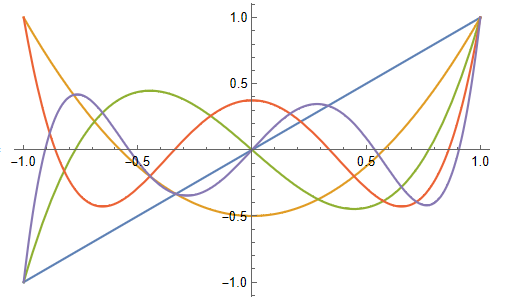
\includegraphics[scale=1]{Captura de pantalla 2023-05-23 032130.png}
    \caption{Polinomios de Legendre normalizados}
    \label{legendre}
\end{figure}
 \end{obs}
 \begin{ejem}[\textbf{Cuadratura de Gauss-Legendre de dos puntos}]
Utilizando la fórmula de recurrencia calculamos $p_2(x)$:
$$p_o=1$$
$$p_1=(x-\alpha_1)p_o$$
$$\alpha_1=\dfrac{\int_{-1}^1xdx}{\int_{-1}^1 dx}=0\Rightarrow p_1=x$$
$$p_2=(x+\alpha_2)p_1-\gamma_2^2p_o$$
$$\gamma_2^2=\dfrac{\int_{-1}^1x^2dx}{\int_{-1}^1 dx}=\dfrac{1}{3}\qquad \alpha_2=\dfrac{\int_{-1}^1x^3dx}{\int_{-1}^1x^2dx}=0\Rightarrow p_2=x^2-\dfrac{1}{3}$$
Los nodos de la cuadratura serán por tanto $x_1=\dfrac{1}{\sqrt{3}}$ y $x_2=-\dfrac{1}{\sqrt{3}}$. Calculemos ahora los pesos de la cuadratura utilizando (\ref{pesos:gauss}):
$$\omega_1=\dfrac{\int_{-1}^1p_1^2dx}{p_1(x_1)p'_2(x_1)}=\dfrac{\frac{2}{3}}{\frac{1}{\sqrt{3}}\cdot \frac{2}{\sqrt{3}}}=1$$
$$\omega_2=\dfrac{\int_{-1}^1p_1^2dx}{p_1(x_2)p'_2(x_2)}=\dfrac{\frac{2}{3}}{\frac{-1}{\sqrt{3}}\cdot \frac{-2}{\sqrt{3}}}=1$$
Obteniendo por tanto la fórmula
\begin{align}
\int_{-1}^1f(x)dx\approx f\left(\dfrac{1}{\sqrt{3}}\right)+f\left(-\dfrac{1}{\sqrt{3}}\right)
\label{legendre:2}
\end{align}
que será exacta para polinomios de grado menor o igual que $3$ (tan exacta como la fórmula de Simpson).
\end{ejem}
\begin{ejem}[\textbf{Cuadratura de Gauss-Legendre de tres puntos}]
Para $n=3$ los nodos de cuadratura serán las raíces de $p_3$
$$p_3(x)=(x-\alpha_3)p_2(x)-\gamma_3^2p_1(x)$$
donde
$$\alpha_3=\dfrac{g_{\omega}(p_2,xp_2)}{g_{\omega}(p_2,p_2)}=-\dfrac{\displaystyle\int_{-1}^1p_2(x)^2\cdot x dx}{\displaystyle\int_{-1}^1p_2(x)^2dx}$$
observemos que
$$\int_{-1}^1p_2(x)\cdot p_2(x)\cdot xdx=\int_{-1}^1p_2(x)\left(x^2-\dfrac{1}{3}\right)x=\int_{-1}^1p_2(x)\cdot x^3dx=0$$
dado que el grado del polinomio del integrando es impar, con lo cual $\alpha_3=0$. Por otro lado:
$$\gamma_3^2=\dfrac{\displaystyle\int_{-1}^1p_2(x)^2dx}{\displaystyle\int_{-1}^1p_1(x)^2dx}=\dfrac{\displaystyle \int_{-1}^1\left(x^2-\dfrac{1}{3}\right)x^2dx}{\frac{2}{3}}=\dfrac{\nicefrac{2}{5}-\nicefrac{2}{9}}{\nicefrac{2}{3}}=\dfrac{4}{15}$$
Concluyendo entonces que
$$p_3(x)=xp_2-\dfrac{4}{15}p_1=x\left(x^2\left(\dfrac{1}{3}+\dfrac{4}{15}\right)\right)=x\left(x^2-\dfrac{3}{5}\right)$$
Y por tanto los nodos de integración serán $x_1=-\sqrt{\dfrac{3}{5}},\,x_2=0\, ,x_3=\sqrt{\dfrac{3}{5}}$. Calculemos ahora los pesos resolviendo el siguiente sistema:
$$\omega_1+\omega_2+\omega_3=g_{\omega}(p_o,p_o)=2$$
$$\omega_1p_1(x_1)+\omega_2p_1(x_2)+\omega_3p_1(x_3)=0$$
$$\omega_1p_2(x_1)+\omega_2p_2(x_2)+\omega_3)p_2(x_3)=0$$
Sustituyendo $x_1=-x_3$ en la primera ecuación obtenemos
$$\omega_2=2-2\omega_1$$
Como $p_1(x)=x$ y $x_1=-x_3$ por la segunda ecuación tenemos que 
$$\omega_1x_1-\omega_3x_1=0\Rightarrow\omega_1=\omega_3$$
Usando esto en la tercera ecuación y dando valores a los nodos tenemos que
$$2\omega_1\left(\dfrac{3}{5}-\dfrac{1}{3}\right)+\omega_2\left(-\dfrac{1}{3}\right)=0$$
$$2\omega_1\left(\dfrac{4}{15}\right)+(2-2\omega_1)\left(-\dfrac{1}{3}\right)=0$$
$$\dfrac{18}{15}\omega_1=\dfrac{2}{3}$$
Despejando obtenemos que $\omega_1=\omega_3=\dfrac{5}{9}$ y con lo cual $\omega_2=\dfrac{8}{9}$, obteniendo por tanto la fórmula
\begin{align}
 \int_{-1}^1f(x)dx\approx\dfrac{5}{9}\cdot f\left(\sqrt{\dfrac{3}{5}}\right)+ \dfrac{8}{9}\cdot f(0)+\dfrac{5}{9}\cdot f\left(\sqrt{\dfrac{3}{5}}\right) 
 \label{legendre:3}
\end{align}

\end{ejem}

\subsection{Fórmula de cuadratura de Gauss-Chebyshev}
\begin{defin}
Las \textbf{cuadraturas de Gauss-Chebyshev} son formas de cuadratura gaussiana con $[a,b]=[-1,1]$ y $\omega(x)=\dfrac{1}{\sqrt{1-x^2}}$. Esto es, fórmulas para aproximar integrales de la forma
$$\int_{-1}^1\dfrac{f(x)}{\sqrt{1-x^2}}dx$$
\end{defin}
\begin{obs}
Haciendo el cambio de variable $x=\cos\theta$ obtenemos lo siguiente
$$\int_{-1}^1\dfrac{f(x)}{\sqrt{1-x^2}}dx=-\int_{\pi}^0f(\cos\theta)\cdot \dfrac{\sin\theta}{\sqrt{1-\cos^2\theta}}d\theta=\int_0^\pi f(\cos\theta)d\theta$$  
\end{obs}
\begin{lem}
Los polinomios de Chebyshev $T_n$ son ortogonales para la norma
$$g_{\omega}(p,q)=\int_{-1}^1\dfrac{p(x)q(x)}{\sqrt{1-x^2}}dx$$
\end{lem}
\begin{dem}
Como $T_i(x)=\cos(i\cdot \arccos(x))$ se tiene que
$$g_{\omega}(T_i,T_j)=\int_{-1}^1\dfrac{T_i(x)T_j(x)}{\sqrt{1-x^2}}=\int_0^{\pi}\cos(i\theta)\cos(j\theta)d\theta$$
Si sumamos las dos siguientes identidades
$$\cos(i\theta+j\theta)=\cos(i\theta)\cos(j\theta)-\sin(i\theta)\sin(j\theta)$$
$$\cos(i\theta-j\theta)=\cos(i\theta)\cos(j\theta)+\sin(i\theta)\sin(j\theta)$$
obtenemos que
$$\cos(i\theta)\cos(j\theta)=\dfrac{\cos(i\theta+j\theta)+\cos(i\theta-j\theta)}{2}$$
Sustituyendo esto en la integral obtenemos lo siguiente:
$$g_\omega(T_i,T_j)=\dfrac{1}{2}\int_0^{\pi}\cos((i+j)\theta)+\dfrac{1}{2}\int_0^{\pi}\cos((i-j)\theta)=0$$
siempre que $i\neq j$.
\qed\end{dem}
\begin{cor}
Los nodos de la cuadratura serán por tanto los nodos de Chebyshev
$$x_k=\cos\left(\dfrac{2k-1}{2n}\pi\right)$$
con $k=1,\ldots,n$
\end{cor}
\begin{prop}[\textbf{Fórmula de cuadratura de Gauss-Chebyshev}] Si $x_i$ son los nodos de Chebyshev, la fórmula
\begin{align}
 \int_{-1}^1\dfrac{f(x)}{\sqrt{1-x^2}}dx\approx\dfrac{\pi}{n}\sum_{i=1}^nf(x_i)
 \label{gauss:cheb}
\end{align}
es exacta para los polinomios de grado menor o igual que $2n-1$.
\end{prop}
\begin{dem}
Sabemos que para que la cuadratura
$$\int_{-1}^1\dfrac{f(x)}{\sqrt{1-x^2}}dx\approx\sum_{i=1}^n\omega_if(x_i) $$
sea exacta para polinomios de grado menor o igual que $2n-1$ los nodos de la cuadratura tienen que ser los nodos de Chebyshev. Para calcular los pesos con la fórmula (\ref{pesos:gauss}) debemos tener en cuenta que los polinomios $T_n(x)$ no son mónicos, esto es, $p_n=2^{1-n}\cdot T_n$. De esta forma:
$$\omega_i=\dfrac{g_\omega(2^{2-n}\cdot T_{n-1},2^{2-n}\cdot T_{n-1})}{2^{1-n}\cdot T'_n(x_i)\cdot 2^{2-n}T_{n-1}(x_i)}=\dfrac{2^{4-2n}}{2^{3-2n}}\cdot \dfrac{g_\omega(T_{n-1},T_{n-1})}{T'_n(x_i)\cdot T_{n-1}(x_i)}= 2\cdot  \dfrac{g_\omega(T_{n-1},T_{n-1})}{T'_n(x_i)\cdot T_{n-1}(x_i)}  $$
Calculemos entonces $\dfrac{dT_n(x)}{dx}$, tomando $x=\cos\theta$
$$\dfrac{dT_n(x)}{dx}=\dfrac{dT_n(\theta)}{d\theta}\cdot \dfrac{d\theta}{dx}=\dfrac{d}{d\theta}(\cos(n\theta))\cdot\dfrac{-1}{\sqrt{1-\cos^2\theta}}=\dfrac{n\sin(n\theta)}{\sin\theta}$$
Con lo cual
$$T'_{n}(x_i)\cdot T_{n-1}(x_i)=\dfrac{n\sin\left(n\cdot\dfrac{2i-1}{2n}\pi\right)}{\sin\left(\dfrac{2i-1}{2n}\pi\right)}\cdot \cos\left(((n-1)\dfrac{2i-1}{2n}\pi\right)=$$
$$=\dfrac{n\sin\left(\dfrac{2i-1}{2}\pi\right)}{\sin\left(\dfrac{2i-1}{2n}\pi\right)}\cdot\left(\cos\left(\dfrac{2i-1}{2}\pi\right)\cdot \cos\left(-\dfrac{2i-1}{2n}\pi\right)+\sin\left(\dfrac{2i-1}{2}\pi\right)\cdot \sin\left(\dfrac{2i-1}{2n}\pi\right)\right)=$$
$$=\dfrac{n\sin\left(\dfrac{2i-1}{2}\pi\right)}{\sin\left(\dfrac{2i-1}{2n}\pi\right)}\cdot\left(\cos\left(i\pi-\dfrac{\pi}{2}\right)\cdot \cos\left(-\dfrac{2i-1}{2n}\pi\right)+\sin\left(\dfrac{2i-1}{2}\pi\right)\cdot \sin\left(\dfrac{2i-1}{2n}\pi\right)\right)=$$
$$=\dfrac{n\sin\left(\dfrac{2i-1}{2}\pi\right)}{\sin\left(\dfrac{2i-1}{2n}\pi\right)}\cdot\left(\sin\left(i\pi\right)\cdot \cos\left(-\dfrac{2i-1}{2n}\pi\right)+\sin\left(\dfrac{2i-1}{2}\pi\right)\cdot \sin\left(\dfrac{2i-1}{2n}\pi\right)\right)=$$
$$=n\cdot \sin^2\left(\dfrac{2i-1}{2}\pi\right)=n$$
Calculemos ahora el numerador:
$$g_{\omega}(T_{n-1},T_{n-1})=\int_{-1}^1\dfrac{T_{n-1}(x)^2}{\sqrt{1-x^2}}dx=\int_{-1}^1\cos^2((n-1)\theta)=\int_{-1}^1\dfrac{1+\cos(2(n-1)\theta)}{2}=\dfrac{\pi}{2}$$
Reuniendo los resultados anteriores, podemos concluir que
$$\omega_i=\dfrac{\pi}{n}$$
\qed\end{dem}
\subsection{Error de las cuadraturas gaussianas}
\begin{prop}
El error de la fórmula de cuadratura gaussiana
$$\int_a^bf(x)\omega(x)dx\approx\sum_{i=1}^n\omega_if(x_i)$$
viene dado por la expresión
\begin{align}
 \mathcal{E}_G=\dfrac{f^{(2n)}(\xi)}{(2n)!}g_{\omega}(p_n,p_n)
 \label{error:gauss}
\end{align}
\end{prop}
\begin{dem}
 Como siempre, tenemos que calcular
 $$\mathcal{E}=\int_a^bf(x)\omega(x)dx-\sum_{i=1}^n\omega_if(x_i)$$
 Sea ahora $H(x)$ el polinomio de interpolación de Hermite de $f(x)$ correspondiente a los pares $\{(x_1,\alpha_1),\ldots,(x_n,\alpha_n)\}$. Queremos que el grado del polinomio sea máximo, esto es, de grado $2n-1$, con lo cual:
 $$\sum_{i=1}^n\alpha_1+n-1=2n-1\Longrightarrow\sum_{i=1}^n\alpha_i=n$$
 Luego tomando $\alpha_i=1$ tenemos que $H(x)$ es de grado $2n-1$. De esta forma:
 $$\int_a^bf(x)\omega(x)dx-\sum_{i=1}^n\omega_if(x_i)=\int_a^bf(x)\omega(x)dx-\sum_{i=1}^n\omega_iH(x_i)=
 \int_a^bf(x)\omega(x)dx-\int_{a}^bH(x)\omega(x)dx=$$
 $$=\int_a^b(f(x)-H(x))\omega(x)dx$$
 Y por la fórmula del error de la interpolación de Hermite (\ref{error:herm})
 $$\mathcal{E}=\int_a^b\dfrac{f^{(2n)}(\xi)}{(2n)!}\prod_{i=1}^n(x-x_i)^2\omega(x)dx=$$
 $$=\dfrac{f^{(2n)}(\xi)}{(2n)!}\int_a^b\prod_{i=1}^n(x-x_i)^2\omega(x)dx=\dfrac{f^{(2n)}(\xi)}{(2n)!}g_{\omega}(p_n,p_n)$$
 donde hemos empleado que $p_n(x)=\prod_{i=1}^n(x-x_i)$ por ser una cuadratura gaussiana.
\qed\end{dem}
\subsection{Cálculo efectivo de los nodos y los pesos}
\begin{obs}
Los métodos numéricos para calcular los autovalores de matrices son más estables que los que calculan las raíces de polinomios. Por esta razón, desarrollaremos un método matricial para calcular los nodos y los pesos de las cuadraturas gaussianas.
\end{obs}
\begin{met}[\textbf{de Golub-Welsch}]
Si $p_o,\ldots,p_n$ son los polinomios ortogonales de la cuadratura, sabemos que están relacionados por la fórmula
$$p_{i+1}=(x-\alpha_{i+1})p_i(x)-\gamma_{i+1}^2p_{i+1}(x)$$
de esta forma
$$xp_i(x)=\gamma_{i+1}^2p_{i-1}+\alpha_ip_i(x)+p_{i+1}$$
luego si $x_i$ son los nodos de la cuadratura
$$x_i\cdot\left(\begin{array}{c}
     p_o(x_i) \\
      p_1(x_i)\\
      \vdots\\
      p_{n-1}
\end{array}\right)=\left(\begin{array}{cccc}
     \alpha_1&1&\cdots&0 \\
      \gamma_2^2&\alpha_2&\ddots&\vdots\\
      \vdots&\ddots&\ddots&1\\
      0&\cdots&\gamma_n^2&\alpha_n
\end{array}\right)\cdot \left(\begin{array}{c}
     p_o(x_i) \\
      p_1(x_i)\\
      \vdots\\
      p_{n-1}(x_i)
\end{array}\right) $$
Si tomamos
$$e=\left(\begin{array}{c}
     p_o(x_i) \\
      p_1(x_i)\\
      \vdots\\
      p_{n-1}(x_i)
\end{array}\right)\qquad \tilde{J}_n=\left(\begin{array}{cccc}
     \alpha_1&1&\cdots&0 \\
      \gamma_2^2&\alpha_2&\ddots&\vdots\\
      \vdots&\ddots&\ddots&1\\
      0&\cdots&\gamma_n^2&\alpha_n
\end{array}\right)$$
tenemos que $\tilde{J}_n e=x_i\cdot e$, esto es, $e$ es un valor propio de $\tilde{J}_n$ de valor propio $x_i$. Vamos a hacer un cambio de base diagonal de tal forma que la matriz de $\tilde{J}_n$ sea simétrica, esto es
$$J_n=D^{-1}\cdot \tilde{J}_n\cdot D$$
$$D=\left(\begin{array}{cccc}
     \lambda_1&0&\cdots&0 \\
      0&\lambda_2&\ddots&\vdots\\
      \vdots&\ddots&\ddots&0\\
      0&\cdots&0&\lambda_n
\end{array}\right)\qquad J_n=\left(\begin{array}{cccc}
     \alpha_1&\gamma_2&\cdots&0 \\
      \gamma_2&\alpha_2&\ddots&\vdots\\
      \vdots&\ddots&\ddots&\gamma_n\\
      0&\cdots&\gamma_n&\alpha_n
\end{array}\right)$$
Queremos entonces que se verifique que $$(\tilde{J}_n\cdot D )e_i=(D\cdot J_n)e_i$$ para todos los vectores $e_i$ de la base estándar de $\mathbb{R}^n$. Por un lado tenemos que
$$(D\cdot J_n)e_i=D(\gamma_{i-1}+\alpha_ie_i+\alpha_{i+1}e_{i+1})=\lambda_{i-1}\gamma_i e_{i-1}+\lambda_i\alpha_i e_i+\lambda_{i+1}\gamma_{i+1} e_{i+1}$$
y por otro que
$$(\tilde{J}_n\cdot D )e_i=\tilde{J}_n(\lambda_ie_i)=\lambda_i e_{i-1}+\lambda_i\alpha_i e_i+\lambda_i\gamma_{i+1}^2 e_{i+1}$$
Si igualamos los coeficientes podemos concluir que
$$\lambda_i= \gamma_i\cdot \lambda_{i-1}=\gamma_{i}\cdot \gamma_{i-1}\cdot\lambda_{i-2}=\cdots=\gamma_2\cdot \ldots \cdot \gamma_i\cdot \lambda_1$$
donde tomaremos $\lambda_1=1$ por ser arbitrario. Reuniendo estos resultados deducimos que los vectores
$$\tilde{v}^{(i)}=D^{-1} e= \left(\begin{array}{c}
     \nicefrac{1}{\lambda_1}\cdot p_o(x_i) \\
     \nicefrac{1}{\lambda_2}\cdot p_1(x_i)\\
      \vdots\\
     \nicefrac{1}{\lambda_n}\cdot p_{n-1}(x_i)
\end{array}\right)\qquad \lambda_i= \gamma_2\cdot \ldots \cdot \gamma_i$$
son vectores propios de $J_n$ de valor propio $x_i$ ya que
$$J_n(D^{-1}e)=(D^{-1}\cdot \tilde{J}_n\cdot D)(D^{-1}e)=D^{-1}\cdot \tilde{J}_n e=D^{-1}(x_i\cdot e)=x_i\cdot (D^{-1}e)$$
Podemos emplear lo deducido anteriormente para calcular los pesos de las cuadraturas gaussianas como sigue. El sistema que determina los nodos se escribe en la base $\tilde{v}^{(i)}$ como
$$\sum_{i=1}^n \rho_j\cdot p_o(x_i)\omega_i=\left\{ 
\begin{array}{cc}
   g_{\omega}(p_o,p_o)   &  j=0 \\
    0 & j\neq 0 
\end{array}\right.  $$
 con $\rho_o=1$ y $\rho_j=\dfrac{1}{\lambda_{j+1}}$. Si lo escribimos de forma matricial
 $$\left(\begin{array}{c|c|c|c}
      \tilde{v}^{(1)} & \tilde{v}^{(2)} &\cdots & \tilde{v}^{(n)} 
 \end{array}\right)\cdot \left(\begin{array}{c}
     \omega_1 \\
      \omega_2\\
      \vdots\\
      \omega_n
\end{array}\right)=\left(\begin{array}{c}
     g_{\omega}(p_o,p_o) \\
     0\\
      \vdots\\
      0
\end{array}\right) $$
Por ser $J_n$ simétrica y los $x_i$ distintos, sabemos que los $\tilde{v}^{(i)}$ son ortogonales entre sí, esto es, $(\tilde{v}^{(j)})^t\cdot\tilde{v}^{(i)}=\delta_{ij}\cdot \|\tilde{v}^{(i)}\|^2 $. Multiplicando el sistema anterior por $(\tilde{v}^{(i)})^t$ tenemos que
 $$\left(\begin{array}{c|c|c|c}
     )\tilde{v}^{(i)})^t\cdot  \tilde{v}^{(1)} &(\tilde{v}^{(i)})^t\cdot  \tilde{v}^{(2)} &\cdots &(\tilde{v}^{(i)} )^t\cdot \tilde{v}^{(n)} 
 \end{array}\right)\cdot \left(\begin{array}{c}
     \omega_1 \\
      \omega_2\\
      \vdots\\
      \omega_n
\end{array}\right)=(\tilde{v}^{(i)})^t\cdot \left(\begin{array}{c}
     g_{\omega}(p_o,p_o) \\
     0\\
      \vdots\\
      0
\end{array}\right) $$
 $$\left(\begin{array}{c|c|c|c|c}
     0 &\cdots  &\|\tilde{v}^{(i)}\|^2&\cdots&0 
 \end{array}\right)\cdot \left(\begin{array}{c}
     \omega_1 \\
      \omega_2\\
      \vdots\\
      \omega_n
\end{array}\right)=\tilde{v}_1^{(i)}\cdot g_{\omega}(p_o,p_o)
$$
Como $\tilde{v}_1^{(i)}=\dfrac{1}{\lambda_1}\cdot p_o(x_i)=1$, podemos concluir que
$$\omega_i=\dfrac{g_{\omega}(p_o,p_o)}{\|\tilde{v}^{(i)}\|^2}$$
Supongamos ahora que $v^{(i)}$ es otro vector propio  de valor propio $x_i$. Se tiene entonces que
$$v^{(i)}=\mu\cdot \tilde{v}^{(i)}\Rightarrow \|v^{(i)}\|^2=\mu^2\cdot \|\tilde{v}^{(i)}\|^2\Rightarrow \|\tilde{v}^{(i)}\|^2=\dfrac{\|v^{(i)}\|^2}{\mu^2}$$
Sustituyendo esto en la fórmula anterior
$$\omega_i=\dfrac{g_{\omega}(p_o,p_o)}{\|v^{(i)}\|^2}\cdot \mu^2$$
y como $\tilde{v}_1^{(i)}=1$, $\mu=v_1^{i}$. Con este resultado obtenemos el siguiente teorema.
\end{met}
\begin{teo}
Sea $v^{(i)}$ un vector propio de $J_n$ con valor propio $x_i$ y tal que $\|v^{(i)}\|^2=g_{\omega}(p_o,p_o)$. Entonces, los pesos de la cuadratura gaussiana son
$$\omega_i=(v_1^{(i)})^2$$
\end{teo}
\section{Ejercicios}
\begin{ejer}
Calcula $\ln(2)$ con un error menor que $0.01$ utilizando el método de Simpson compuesto aplicado a la integral
$$\ln(2)=\int_1^2\dfrac{1}{x}dx$$
\end{ejer}
\begin{sol}
Calculemos en primer lugar el número de subvintervalos necesarios para que el error sea menor que $0.001$ utilizando la fórmula del error del método de Simpson compuesto:
$$\dfrac{M_4}{180}\cdot(b-a)\cdot \left(\dfrac{b-a}{2n}\right)^4<0.01$$
donde $M_4=\max|f^{(4)}|$ con $x\in[1,2]$ y $f(x)=\dfrac{1}{x}$. Acotemos por tanto  $f^{(4)}(x)$:
$$f'(x)=-\dfrac{1}{x^2}$$
$$f''(x)=\dfrac{2}{x^3}$$
$$f^{(3)}(x)=-\dfrac{6}{x^4}$$
$$f^{(4)}(x)=\dfrac{24}{x^5}$$
$$f^{(5)}(x)=-\dfrac{120}{x^6}$$
Como $f^{(5)}(x)<0$ y nunca se anula, el máximo de $f^{(4)}(x)$ ocurre en $x=1$, esto es $M_4=|f^{(4)}(1)|=24$. Calculemos a continuación la $n$:
$$\dfrac{24}{180}\cdot(2-1)\cdot \left(\dfrac{2-1}{2n}\right)^4<0.001$$
$$\dfrac{1}{n^4}<0.12$$
$$n>1.7$$
Luego tomaremos $n=2$. Aplicando la fórmula de Simpson compuesta con $h_n=\dfrac{1}{4}$ obtenemos lo siguiente
$$\int_1^2\dfrac{1}{x}dx\approx \dfrac{1}{12}(f(1)+2f(1.5)+4(f(1.25)+f(1.75))+f(2))\approx 0.69325$$
siendo el valor ''real'' de $\ln(2)=0.69314\ldots$
\end{sol}
\begin{ejer}
    Una cuerda vibra adoptando la forma $y=\sin x $, entre las abcisas $x=0$ y $x=4$ en un instante $t_o$. Calcúlese aproximadamente la longitud de la cuerda, utilizando un método numérico con $n=8$. Acotar el error cometido.
\end{ejer}
\begin{sol}
Sabemos que la longitud de la cuerda se puede calcular mediante la integral
$$L=\int_0^4\sqrt{1+(y')^2}=\int_0^4\sqrt{1+\cos^2x}dx$$
Empleemos la fórmula del trapecio compuesto con $n=8$ para aproximar dicha integral. Tendremos entonces que $h_n=\dfrac{4-0}{8}=0.5$ y el integrando será $g(x)=\sqrt{1+\cos^2x}$. Necesitaremos por tanto los siguientes datos:
$$\begin{array}{|c|c|c|c|c|c|c|c|c|}
    \hline
     x_o&x_1&x_2&x_3&x_4&x_5&x_6&x_7&x_8  \\
     0.0&0.5&1.0&1.5&2.0&2.5&3.0&3.5&4.0 \\
     \hline
     g(x_o)&g(x_1)&g(x_2)&g(x_3)&g(x_4)&g(x_5)&g(x_6)&g(x_7)&g(x_8)\\
     1.41421&1.33047&1.13663&1.0025&1.08313&1.28134&1.40715&1.37002&1.18468\\
     \hline
\end{array}$$
Con lo cual:
$$L\approx \dfrac{1}{6}\left(g(x_o)+2\sum_{i=1}^7g(x_i)+g(x_8)\right)\approx 4.9578$$
Analicemos ahora el error de este método:
$$\mathcal{E}\leq \dfrac{M_2}{12}\cdot (b-a)\cdot h_n^2=\dfrac{M_2}{12}\cdot 4\cdot\dfrac{1}{4}=\dfrac{M_2}{12}$$
donde $M_2=\max|g''(x)|$ con $x\in[0,4]$. Acotemos por tanto $g''(x)$:
$$|g''(x)|=\left|\dfrac{\cos(2x)+\cos^4x}{(1+\cos^2x)^{\frac{3}{2}}}\right|\leq \left|\dfrac{1}{(1+\cos^2x)^{\frac{3}{2}}}\right| \cdot (|\cos(2x)|+|\cos^4x|)\leq 1\cdot (1+1)=2 $$
Y con lo cual $M_2\leq 2$, de esta forma:
$$\mathcal{E}\leq\dfrac{2}{12}\approx 0.167$$
\end{sol}
\begin{ejer}
Se desea evaluar la integral
$$I=\int_0^1e^{-x^2}dx$$
por un método de integración numérica con un error menor a $10^{-5}$. Determina el número de subintervalos a considerar en los métodos del trapecio y de Simpson para conseguir dicha precisión.
\end{ejer}
\begin{sol}
Estudiemos en primer luegar el número de subintervalos necesarios para el método del trapecio. Empleando la fórmula del error para este método, sabemos que se debe verificar que
$$\dfrac{M_2}{12}\cdot(b-a)\cdot\left(\dfrac{b-a}{n}\right)^2<10^{-5}$$
$$\dfrac{M_2}{12}\cdot\dfrac{1}{n^2}<10^{-5}$$
$$n>\sqrt{\dfrac{10^{5}\cdot M_2}{12}}$$
donde $M_2=\max|f''(x)|$ con $x\in[0,1]$ y $f(x)=e^{-x^2}$. Calculemos entonces las primeras derivadas de $f(x)$:
$$f'(x)=-2x\cdot e^{-x^2}$$
$$f''(x)=(4x^2-2)e^{-x^2}$$
$$f^{(3)}(x)=-4x(2x^2-3)\cdot e^{-x^2}$$
Como $f^{(3)}(x)$ se anula en $x_1=0$ y en $x_2=\sqrt{\dfrac{3}{2}}$ pero $x_2\nin [0,1]$, los posibles máximos de $|f''(x)|$ son los extremos del intervalo:
$$|f''(0)|=|-2|=2$$
$$|f''(1)|=\dfrac{2}{e}<2$$
Por tanto, $M_2=2$ y se tiene entonces que
$$n>\sqrt{\dfrac{10^{5}\cdot 2}{12}}\approx 129.099$$
Luego para emplear el método del trapecio compuesto necesitaríamos al menos 130 subintervalos.

Analicemos ahora el método de Simpson. Empleando la fórmula del error podemos deducir que
$$\dfrac{M_4}{180}\cdot (b-a)\cdot \left(\dfrac{b-a}{2n}\right)^4<10^{-5}$$
$$\dfrac{M_4}{180}\cdot\dfrac{1}{16n^4}$$
$$n>\sqrt[4]{\dfrac{10^5\cdot M_4}{2880}}$$
donde $M_4=\max|f^{(4)}|$. Acotemos por tanto $|f^{(4)}(x)|$:
$$f^{(4)}(x)=4(4x^4-12x^2+3)\cdot e^{-x^2}$$
$$f^{(5)}(x)=-8x(4x^{4}-20x^2+15)\cdot e^{-x^2}$$
Resolviendo $f^{(5)}(x)=0$ obtenemos los posibles máximos de $|f^{(4)}(x)|$. Además de la solución $x=0$, debemos considerar las soluciones de 
$$4x^4-20x^2+15=0$$
que serán
$$x_1=-\sqrt{\dfrac{5}{2}-\sqrt{\dfrac{5}{2}}} \qquad x_2=\sqrt{\dfrac{5}{2}-\sqrt{\dfrac{5}{2}}} $$
$$x_3=-\sqrt{\dfrac{5}{2}+\sqrt{\dfrac{5}{2}}} \qquad x_4=\sqrt{\dfrac{5}{2}+\sqrt{\dfrac{5}{2}}} $$
Como $x_1,x_3,x_4\nin [0,1]$, debemos considerar los siguientes casos:
$$|f^{(4)}(0)|=12$$
$$|f^{(4)}(x_2)|\approx 7.4194$$
$$|f^{(4)}(1)|\approx 7.3575$$
Y por tanto $M_2=12$, de esta forma
$$n>\sqrt[4]{\dfrac{10^5\cdot 12}{2880}}\approx 4.5180$$
Esto es, necesitaríamos por lo menos $5$ subintervalos para alcanzar la precisión requerida.
\end{sol}
\begin{ejer}
Calcula la integral del problema anterior usando una cuadratura de Gauss con $n=3$. Sabiendo que el resultado ''exacto'' es $I=0.7468241330\ldots$, compara los resultados
\end{ejer}
\begin{sol}
Para emplear la cuadratura de Gaus-Legendre de tres puntos debemos estar trabajando en el intervalo de integración $[-1,1]$. Haciendo el siguiente cambio de variable
$$x=\dfrac{1}{2}-\dfrac{t}{2}$$
$$dx=-\dfrac{1}{2}dt$$
Obtenemos lo siguiente:
$$\int_0^1e^{-x^2}=\int_1^{-1}e^{-\frac{1}{4}(t-1)^2}\cdot \dfrac{-1}{2}dt=\dfrac{1}{2}\int_{-1}^1e^{-\frac{1}{4}(t-1)^2}$$
Si denotamos por $f(t)=e^{-\frac{1}{4}(t-1)^2}$, aplicando la cuadratura de Gauss-Legendre tenemos que
$$I\approx \dfrac{5}{18}\cdot f\left(\sqrt{\dfrac{3}{5}}\right)+ \dfrac{8}{18}\cdot f(0)+\dfrac{5}{18}\cdot f\left(\sqrt{\dfrac{3}{5}}\right)\approx 0.78157$$
Es decir, hemos obtenido un error de menor que $0.1$.
\end{sol}
\begin{ejer}
Calcula la integral
$$I=\int_{-1}^1\dfrac{e^x}{\sqrt{1-x^2}}dx$$
utilizando las cuadraturas de Gauss-Chebyshev correspondientes a $n=2$ y $n=3$. Evalúa el error en ambos casos sabiendo que el resultado ''exacto'' de la integral es $I=3.9774632...$
\end{ejer}
\begin{sol}
Para $n=2$ los nodos de Chebyshev son
$$x_1=\cos\left(\dfrac{\pi}{4}\right)\qquad x_2=\cos\left(\dfrac{3\pi}{4}\right)$$
Por tanto, tomando $f(x)=e^x$ la aproximación obtenida con la cuadratura de Gauss-Chebyshev será
$$I\approx \dfrac{\pi}{2}\left(f\left(\cos\left(\dfrac{\pi}{4}\right)\right)+f\left(\cos\left(\dfrac{3\pi}{4}\right)\right)\right)\approx 3.96027$$
Teniendo por tanto un error menor que $0.1$.

Por otro lado, para $n=3$ los nodos de Chebyshev son
$$x_1=\cos\left(\dfrac{\pi}{6}\right)\qquad x_2=0 \qquad x_3=\cos\left(\dfrac{5\pi}{6}\right)$$
Y la aproximación que obtenemos con la cuadratura de Gauss-Chebyshev es
$$I\approx \dfrac{\pi}{3}\left(f\left(\cos\left(\dfrac{\pi}{6}\right)\right)+f(0)+f\left(\cos\left(\dfrac{5\pi}{6}\right)\right)\right)\approx 3.97732$$
Obteniendo un error menor que $0.001$.
\end{sol}





























































\begin{comment}
 
    Consiste en encontrar f{\'o}rmulas (de cuadratura) de la forma:
    $$\int_a^b f(x) \: dx \approx \sum_{i=0}^n \omega_i \: f(x_i)$$
    donde llamaremos a los $\omega_i$ pesos y a los $x_i$ nodos. 
        \subsection{F{\'o}rmulas de integraci{\'o}n interpolatorias}
        \begin{enumerate}[a)]
            \item Los nodos est{\'a}n prefijados: $x_o=a, \ldots, x_k = a + kh_1, \ldots, x_n=b$ con $h=\dfrac{b-a}{n}$ \\
            \textbf{Ejemplo.} F{\'o}rmulas de Newton-Cotes: hay que calcular los $n+1$ pesos $\omega_i$. Para $n=1$ es la f{\'o}rmula del trapecio (se ven ambas m{\'a}s adelante). 
            \item Calcular los nodos y los pesos para que la precisi{\'o}n sea la mayor posible. Se aproxima $f(x)$ por un polinomio de interpolaci{\'o}n de grado $n$. \\
            
        \end{enumerate}
        \subsection{F{\'o}rmula del error} Como siempre, el error es $$\mc{E}(f)=\int_a^b f(x) \: dx - \sum_{i=0}^n \omega_i \: f(x_i)=\int_a^b f(x) \: dx - \int_a^b p_n(x) dx = \int_a^b (f(x)-p_n(x)) \: dx $$
        $$\mc{E}(f)=\int_a^b \dfrac{f^{(n+1)}(\xi)}{(n+1)!} \prod_{i=0}^n (x-x_i) \: dx$$
        \subsection{F{\'o}rmulas de Newton-Cotes}
        Son las fórmulas de cuadratura obtenidas por la integración de $p_n(x)$ polinomio de interpolación de $f$ en $\{x_o, \ldots, x_n\}$ con $x_i = a + i \: \dfrac{b-a}{n}$. Es decir, $\displaystyle \omega_i = \int_a^b \ell_i (x) \: dx$, y por tanto $\displaystyle \int_a^b p_n(x)\:dx = \sum_{i=0}^n \omega_i \: p_n(x_i)$. Para $n=1$ se tiene
        \subsection{F{\'o}rmula del trapecio}
        Tomemos como intervalo de referencia [-1,1], entonces
        $$\int_{-1}^1 f(t) \: dt \approx \omega_o f(-1) + \omega_1 \: f(1)$$
        Como se ha dicho, 
        $$\omega_o=\int_{-1}^1 \ell_o(t) \: dt = \int_{-1}^1 \dfrac{t-1}{-1-1} \: dt = - \dfrac{1}{2} \int_{-1}^1 (t-1) \: dt = - \dfrac{1}{2} \dfrac{1}{2} (t-1)^2 \Big|_{-1}^1 = - \dfrac{1}{4} (-4) = 1$$
        $$\omega_1 = \int_{-1}^1 \ell_1(t) \: dt = \int_{-1}^1 \dfrac{t+1}{2} \: dt = \dfrac{1}{4}(t+1)^2 = \dfrac{1}{4} \: 4 = 1$$
        Por tanto, $\displaystyle 2 = \int_{-1}^1 dt = f(-1) + f(1)$ \textcolor{red}{NO ENTIENDO EL 2} \\
        \textbf{Proposici{\'o}n.}
        Si $\displaystyle \sum_{i=0}^{n} \omega_i \: f(x_i)$ es una f{\'o}rmula de cuadratura interpolaria exacta para polinomios de grado $\leq n$, en particular
        $$\sum_{i=0}^n \omega_i = b-a = \int_a^b dx$$
        Ahora, para calcular la f{\'o}rmula en un intervalo [$a,b$] arbitrario, hacemos un cambio de coordenadas $x=\dfrac{a+b}{2}+t\:\dfrac{b-a}{2} \Rightarrow dx=\dfrac{b-a}{2} \: dt$, por tanto,
        $$\int_a^b f(x) \: dx= \int_{-1}^1 f\left(\dfrac{a+b}{2}+t\:\dfrac{b-a}{2}\right)\dfrac{b-a}{2} \: dt = \dfrac{b-a}{2} \int_{-1}^1 f\left(\dfrac{a+b}{2}+t\:\dfrac{b-a}{2}\right) \: dt \approx $$
        $$\approx \dfrac{b-a}{2} (f(a)+f(b))$$
            \subsubsection{F{\'o}rmula del error del trapecio}
            Como siempre, el error viene dado por
            $$\mc{E}_T=\int_a^b f(x) \: dx - \dfrac{b-a}{2} (f(a)+f(b)) = \int_a^b \dfrac{f^{(2)}(\xi)}{2} (x-a)(x-b) \: dx =   \hfill $$
            $$=\dfrac{f^{(2)}(\xi)}{2} \int_a^b\left(\dfrac{a+b}{2}+t\:\dfrac{b-a}{2}-a\right) \left(\dfrac{a+b}{2}+t\:\dfrac{b-a}{2}-b\right)\dfrac{a-b}{2} \: dt =\dfrac{f^{(2)}(\xi)}{2} \left( \dfrac{b-a}{2}\right)^3\int_{-1}^{1}(t+1)(t-1)\:dt= $$
            $$ = \dfrac{f^{(2)}(\xi)}{2} \left( \dfrac{b-a}{2}\right)^3\int_{-1}^{1}(t-1)^2\:dt= \dfrac{f^{(2)}(\xi)}{2} \left( \dfrac{b-a}{2}\right)^3 \left( \dfrac{2}{3} - 2 \right) = -2 \dfrac{f^{(2)}(\xi)}{2} \left( \dfrac{b-a}{2}\right)^3 = - \dfrac{f^{(2)}(\xi)}{12} \left( {b-a}\right)^3$$
        \subsection{F{\'o}rmula de Simpson}
        Si $n=2$, aproximamos $f(x)$ por $p_2(x)$ polinomio de interpolaci{\'o}n de $f$ en $a,\frac{a+b}{2}, b$
        $$\int_a^b f(x) \: dx \approx \omega_o f(a) + \omega_1 f\left(\dfrac{a+b}{2}\right) + \omega_2 f(b)$$
        Como antes, tomamos el intervalo de referencia $[-1,1]$,
        $$\omega_o=\int_{-1}^1 \ell_o(t) \: dt = \int_{-1}^1 \dfrac{t(t-1)}{(-1)(-2)} \:dt =\dfrac{1}{2} \int_{-1}^1 (t^2-t) \: dt = \dfrac{1}{3} \hfill$$
        $$\omega_1=\int_{-1}^1 \ell_1(t) \: dt = \int_{-1}^1 \dfrac{(t+1)(t-1)}{(-1)1} = - \int_{-1}^1 (t^2-1) = \dfrac{4}{3}$$
        $$\omega_2=\int_{-1}^1 \ell_2(t) \: dt = \int_{-1}^1 \dfrac{(t+1)t}{2 \cdot 1} \: dt = \dfrac{1}{3}$$
        Por tanto, $\displaystyle \int_{-1}^1 f(t) \: dt = \dfrac{1}{3} (f(-1)+4f(0)+f(1))$. Procediendo como antes por el cambio de variable:
        $$\int_a^b f(x) \: dx = \int_{-1}^1 f\left(\dfrac{a+b}{2}+t\:\dfrac{b-a}{2}\right)\dfrac{b-a}{2} \: dt = \dfrac{b-a}{2} \int_{-1}^1 f\left(\dfrac{a+b}{2}+t\:\dfrac{b-a}{2}\right) \: dt \approx $$
        $$\approx \dfrac{b-a}{2} \dfrac{1}{3} (f(a)+4f\left(\dfrac{a+b}{2}\right)+f(b)) = \dfrac{b-a}{6} (f(a)+4f\left(\frac{a+b}{2}\right)+f(b)) $$
        \subsubsection{Error}
        Podeos observar que interpola de manera exacta a polinomios de grado $\leq 3$.
        $$\mc{E}_S = - \dfrac{1}{90} (b-a)^5 f^{(4)}(\xi)$$
        
        \textbf{Proposici{\'o}n.} Dado el intervalo $[a,b]$, sean $x_o, \ldots, x_{2k}$ dados por $x_i=a+i\:\dfrac{b-a}{2k}$, se tiene que
        $$\bbint_a^b \prod_{i=0}^{2k} (x-x_i) \: dx = 0$$ 
        \textit{Demostraci{\'o}n.} \textcolor{red}{METER}
        
        \textbf{Corolario.}
        La f{\'o}rmula de Newton-Cotes es exacta para los polinomios de grado menor o igual que $2k+1=n+1$. \\
        \textit{Demostraci{\'o}n.}
        \subsection{F{\'o}rmulas compuestas} Para disminuir el error, lo m{\'a}s pr{\'a}ctico es disminuir el tamaño del intervalo; por ejemplo, dividiendo el intervalo en $n$ partes iguales obteniendo las fórmulas de cuadratura compuestas:
        \begin{itemize}
            \item \underline{Trapecio compuesto:} dado $[a,b]$, sean $\{x_o, \ldots, x_n\}$ los puntos $x_i=0+i\:\dfrac{b-a}{n}$. As{\'i}, $$\int_a^b f(x)\: dx = \sum_{i=0}^{n-1} \int_{x_i}^{x_{i+1}} f(x) \: dx \approx \sum_{i=0}^{n-1} \dfrac{b-a}{2n}(f(x_i)+f(x_{i+1})) = $$
            $$=\dfrac{b-a}{2n} \sum_{i=0}^{n-1} (f(x_i)+f(x_{i+1}))= \dfrac{b-a}{2n} \left( f(a) + 2 \sum_{i=0}^{n-1} f(x_i) + f(b) \right) $$
            Error:
            $$\int_{x_i}^{x_{i+1}} f(x) \: dx - \dfrac{x_{i+1}-x_i}{2}(f(x_i)+f(x_{i+1}))=-\dfrac{f^{(2)}(\xi_i)}{12}(x_{i+1}-x_i)^3= -\dfrac{f^{(2)}(\xi_i)}{12} \left( \dfrac{b-a}{n} \right)^3$$
            Luego 
            $$\int_a^b f(x) \: dx - \dfrac{b-a}{2n} \left( f(a)+2 \sum_{i=0}^{n-1} f(x_i) + f(b) \right) = \sum_{i=0}^{n-1} -\dfrac{f^{(2)}(\xi_i)}{12} \left(\dfrac{b-a}{n}\right)^3=$$
            $$=-\dfrac{1}{12} \left(\dfrac{b-a}{n}\right)^3 \sum_{i=0}^{n-1} f^{(2)}(\xi_i) = -\dfrac{ f^{(2)}(\xi_i)}{12} n \: \left(\dfrac{b-a}{n}\right)^3 =  -\dfrac{f^{(2)}(\xi_i)}{12} n \: \left(b-a\right) h_n^2$$
            donde $h_n = \dfrac{b-a}{n}$
            \item \underline{M{\'e}todo de Simpson compuesto:} dado el intervalo $I=[a,b]$, sean $x_i=a+i\:\dfrac{b-a}{n}$ con $i=0,\ldots, n$
            $$\int_a^b f(x)\: dx = \sum_{i=0}^{n-1} \int_{x_i}^{x_{i+1}} f(x) \:dx \approx \sum_{i=0}^{n-1} \dfrac{1}{6} \dfrac{b-a}{n} \left( f(x_i) + f\left(\dfrac{x_i+x_{i+1}}{2} \right)+ f(x_{i+1})\right)$$
            $$\int_a^b f(x)\: dx \approx \dfrac{b-a}{6n} \left( f(a) + 2 \sum_{i=0}^{n-1} f(x_i) + 4 \sum_{i=0}^{n-1} f\left(\dfrac{x_i+x_{i+1}}{2} \right) + f(b)\right)$$
            Adem{\'a}s, $\dfrac{x_i+x_{i+1}}{2} = \dfrac{1}{2} \left( a+i\:\dfrac{b-a}{n}+a+(i+1)\dfrac{b-a}{n} \right) = a+(2i+1)\dfrac{b-a}{2n}=a+j\:\dfrac{b-a}{2n}$. Si 
            $y_j=a+j\:\dfrac{b-a}{2n}=\left\{ \begin{array}{ll}
               x_i & \text{ si } j=2i (\text{par}) \\
               \dfrac{x_i+x_{i+1}}{2} & \text{ si } j=2i+1 (\text{impar})
            \end{array}\right.$ y la f{\'o}rmula de Simpson compuesta quedar{\'i}a
            $$I \approx \dfrac{1}{3} h_n  \left( f(a) + 2 \sum_{i=0}^{n-1} f(y_{2i}) + 4 \sum_{i=0}^{n} f\left(y_{2i+1} \right) + f(b)\right)$$
            con $h_n=\dfrac{b-a}{2n}$ y $x_i=a+i \: \dfrac{b-a}{3}, \; y_j=a+j\:\dfrac{b-a}{6}=a+j\: h_3$\\
            Error: 
            $$\int_{x_i}^{x_{i+1}} f(x) \: dx - \dfrac{x_{i+1}-x_i}{6} \: \left(f(x_i)+4 f\left(\dfrac{x_i+x_{i+1}}{2}\right) + f(x_{i+1})\right) = - \dfrac{f^{(4)}(\xi_i)}{90} (x_{i+1}-x_i)^5$$
            de manera que sumando todos los errores en cada intervalo, el error total ser{\'a}:
            $$\sum_{i=0}^{n-1} - \dfrac{f^{(4)}(\xi_i)}{90} \left(\dfrac{b-a}{2n}\right)^5 =- \dfrac{f^{(4)}(\xi)}{90} n \: \left(\dfrac{b-a}{2n}\right)^5 = - \dfrac{f^{(4)}(\xi)}{90}\: \left(\dfrac{b-a}{2}\right) \:  h_n^4 = - \dfrac{f^{(4)}(\xi)}{180}\: (b-a) \:  h_n^4$$
        \end{itemize}
        \subsection{Cuadraturas adaptativas}
        Se trata de adoptar los intervalos de integraci{\'o}n en las caracter{\'i}sticas de la funci{\'o}n a integrar. La idea clave es la de estudiar el error cometido comparando dos integrales num{\'e}ricas consecutivas. \\
        Sea $Q$ una f{\'o}rmula de cuadratura tal que 
        $$I = I_1 + I_2 = \int_{a}^{\frac{a+b}{2}} f(x) \: dx + \int_{\frac{a+b}{2}}^{b} f(x) \: dx = Q_1 + Q_2 + f^{(k)}(\xi_1) \: C(\nicefrac{h}{2})^{k+1}+f^{(k)}(\xi_2) \: C(\nicefrac{h}{2})^{k+1} = $$
        $$=Q_1 + Q_2 + C \: \dfrac{h^{k+1}}{2^k} \: \left( \dfrac{f^{(k)}(\xi_1)+f^{(k)}(\xi_2)}{2}\right) = Q_1 + Q_2 +  f^{(k)}(\Bar{\xi}) C\dfrac{h^{k+1}}{2^k} \: $$
        Si $f^{(k)}(\xi) \approx f^{(k)}(\bar{\xi})$, entoces restando se tiene
        $$0 \approx (Q_1+Q_2) - Q + f^{(k)}(\bar{\xi}) C \: \dfrac{h^{k+1}}{2^k} (1-2^k) \; \Rightarrow \; f^{(k)}(\bar{\xi}) C \: \dfrac{h^{k+1}}{2^k} \approx \dfrac{Q_1+Q_2-Q}{2^k-1}$$
        Si $\dfrac{Q_1+Q_2-Q}{2^k-1}< \varepsilon$, para un $\varepsilon$ dado, la aproximaci{\'o}n que hemos hecho es suficientemente buena: $I \approx Q_1 + Q_2 + \dfrac{Q_1+Q_2-Q}{2^k}$. Si no es suficientemente buena, añadimos el punto $\dfrac{a+b}{2}$ a los que teníamos $[a,b] \rightsquigarrow [a,\frac{a+b}{2}, b]$ y repetimos con los dos primeros:
        $$I=\int_a^{\frac{a+b}{2}} f(x)\: dx=Q+f^{(k)}(\xi) \: C \: h^{k+1} $$
        Si $\dfrac{Q_1+Q_2-Q}{2^k-1} < \varepsilon \: \dfrac{\frac{a+b}{2}-a}{b-a}=\dfrac{\varepsilon}{2}$, se acepta la estimaci{\'o}n de la primera parte $\int_a^{\frac{a+b}{2}} f(x)\: dx$. 
        \subsection{F{\'o}rmulas de cuadratura gaussiana}
        Sea $\omega(x)$ una funci{\'o}n positiva en el intervalo $[a,b]$, las f{\'o}rmulas de cuadratura gaussiana aproximan las integrales
        $$\int_a^b f(x) \: \omega(x) \: dx \approx \sum_{i=1}^n W_i \: f(x_i)$$
        donde llamaremos funci{\'o}n peso a $\omega(x)$ y pesos a los $W_i$, de forma que la cuadratura ser{\'a} exacta para los polinomios de grado menor o igual que $2n-1$. \\
       
        \subsubsection{C{\'a}lculo de los nodos y los pesos}
        Supongamos que tenemos ya la f{\'o}rmula de cuadratura $\displaystyle \int_a^b f(x) \: dx \approx \sum_{i=0}^n \omega_i \: f(x_i)$ exacta para los polinomios de grado menor o igual que $2n-1$. Con los nodos $x_1, \ldots, x_n$ construimos el polinomio de grado $n$, m{\'o}nico $\displaystyle p_n(x)=\prod_{i=1}^n (x-x_i)$. Entonces, $\forall \: q_m(x)$ polinomio de grado menor o igual que $n-1$, se tiene que $$\int_a^b p_n(x) \cdot q_m(x) \; \omega(x) \: dx = \sum_{i=1}^{n} W_i \: p_n(x_i) \: q_m(x_i) = 0$$
        Definimos en $\mathbb{R}[x]$ el producto escalar $\displaystyle g_{\omega}(p,q)=\int_a^b p(x) \: q(x) \: dx$, $p_n(x)$ es ortogonal para este producto escalar a todos los polinomios de grado $\leq n-1$, $p_n(x) \in \mathbb{P}_n(x)$, $p_n(x) \in \mathbb{P}_{n-1}(x)^{\perp}$. Este $p(x)$ existe y es {\'u}nico. Podemos construir entonces los polinomios $\{p_n\}$ utilizando t{\'e}cnicas similares al m{\'e}todo de Gram-Schmidt:
        $$p_o=1 ; \; p_1(x) = x+ \alpha\: ; \; g_{\omega}(p_o,p_1)=\int_a^b (x+\alpha)\: \omega(x) \: dx=0 \; \Rightarrow \; \alpha=\dfrac{-\int_a^b x \: \omega(x) \: dx}{\int_a^b \omega(x) \: dx} $$
        Supongamos construidos los polinomios hasta el grado $n, p_o, p_1, \ldots, p_n$ y construyamos $p_{n+1}$:
        $$p_{n+1}(x)=(x-\alpha_{n+1})p_n(x)+q_{n-1}(x)=(x-\alpha_{n+1})p_n(x)+\sum_{i=0}^{n-1} \beta_i \: p_i (x)$$
        y los coeficientes $\beta_o, \ldots, \beta_{n-1}, \alpha_{n+1}$ se determinan con las condiciones $g_{\omega}(p_{n+1},p_j)=0$ con $j=0,\ldots,n$
        $$g_{\omega}(p_{n+1},p_j)=g_{\omega}((x-\alpha_{n+1})p_n+q_{n-1},p_j)=g_{\omega}(x \: {p_n},p_j)-\alpha_{i+1} \: g_{\omega}(p_{n},p_j) + g_{\omega}(q_{n-1},p_j)$$
        
        \subsection{Polinomios de Legendre} Los nodos de la cuadratura $\displaystyle \int_a^b f(x) \: \omega(x) \: dx \approx \sum_{i=1}^n W_i \: f(x_i)$ verifican que $\displaystyle p_n(x)=\prod_{i=1}^n (x-x_i)$. Es decir, los polinomios $p_n$ (asociados a los nodos de cuadratura) est{\'a}n caracterizados por $p_n(x)$ es m{\'o}nico y $<p_n> = \mathbb{P}_{n-1}(x)^{\perp}$ en $\mathbb{P}_n(x)$.
        
        Lo siguiente que vamos a ver es c{\'o}mo se pueden escribir $p_{n+1}(x)$ en funci{\'o}n de $p_n(x), \ldots, p_o(x)$
        
        Si dividimos $p_{n+1}(x)$ entre $p_n(x)$:
        $$p_{n+1}(x)=(x-\delta_{n+1}) p_n + q_{n-1}(x) = (x-\delta_{n+1}) p_n +  \sum_{i=0}^{n-1} \beta_i \: p_i(x)$$
        porque $\{p_o, \ldots, p_n\}$ es base de $\mathbb{P}_n(x)$. Los coeficientes $\delta_{n+1}, \beta_o, \ldots, \beta_{n-1}$ se determinan con las igualdades $g_{\omega}(p_{n+1}, p_j)=0$ con $j=0,\ldots,n$; 
        $$0=g_{\omega}(p_{n+1}, p_j)=g_{\omega}\left((x-\delta_{n+1}) p_n +  \sum_{i=0}^{n-1} \beta_i \: p_i(x),p_j \right) = g_{\omega}(x \: p_n,p_j)-\delta_{n+1}\: g_{\omega}(p_n,p_j) + \sum_{i=0}^{n-1} \beta_i \: g_{\omega}(p_i,p_j) = $$
        $$=g_{\omega}(p_n,x \: p_j) - \delta_{n+1} \: g_{\omega}(p_n,p_j) + \sum_{i=0}^{n-1} \beta_i \: g_{\omega}(p_i,p_j)$$
        Luego se tiene que para
        \begin{itemize}
            \item \underline{$j < n-1$} \; $0 = 0 - 0 -\beta_j g_{\omega}(p_j,p_j) \; \Rightarrow \; \beta_j = 0$
            \item \underline{$j=n-1$} \; $g_{\omega}(p_n,x \: p_j) - \delta_{n+1} \: g_{\omega}(p_n,p_{n-1}) + \beta_{n-1} \: g_{\omega}(p_n,p_{n-1}) \; \Rightarrow \; \beta_{n-1}=-\dfrac{g_{\omega}(p_n,p_{n})}{g_{\omega}(p_{n-1},p_{n-1})} = -\gamma_{n+1}^2$ 
            \item \underline{$j=n$} \; $g_{\omega}(p_n,x \: p_n) - \alpha_{n+1} \: g_{\omega}(p_n,p_n) + \gamma_{n+1}^2 \: g_{\omega}(p_{n-1},p_{n}) \; \Rightarrow \; \alpha_{n+1} = \dfrac{g_{\omega}(p_n,x \: p_{n})}{g_{\omega}(p_{n-1},p_{n-1})}$
        \end{itemize}
        En resumen, 
        $$p_{n+1}(x)=(x-\alpha_{n+1}) p_n + \gamma_{n+1}^2 p_{n-1} \quad \alpha_{n+1}= \dfrac{g_{\omega}(p_n,x \: p_{n})}{g_{\omega}(p_{n},p_{n})} \quad \gamma_{n+1}^2 = \dfrac{g_{\omega}(p_n,p_{n})}{g_{\omega}(p_{n-1},p_{n-1})}$$
        
        \textbf{Teorema.} Las ra{\'i}ces de $p_n(x)$ son reales, distintas y contenidas en $[a,b]$
        
        \textit{Demostraci{\'o}n.} Sea $\ell$ el n{\'u}mero de ra{\'i}ces reales contenidas en $[a,b]$ y con multiplicidad impar y sean $a < x_1 < \cdots < x_{\ell} < b$ ra{\'i}ces de $p_n(x)$ con multiplicidad impar. Sea $\displaystyle q_{\ell}(x) = \prod_{i=1}^{\ell} (x-x_i)$, que divide a $p_n(x)$, $p_n(x)=c_{n-\ell} (x) \: q_{\ell}(x)$ con $\displaystyle c_{n-\ell} (x) = \prod_{i=\ell+1}^n (x-x_i)$, de manera que 
        $$\int_a^b p_n(x) \: q_{\ell}(x) \: \omega(x) \: dx = \int_a^b c_{n-\ell} (x) \: q_{\ell} (x)^2 \: \omega(x) \: dx \neq 0$$
        Como $p_n(x)$ es ortogonal a polinomios de grado $< n$, luego $n = \ell$ 
        \subsubsection{C{\'a}lculo de los pesos}
        
        \textbf{Definici{\'o}n.} Las funciones $\{\varphi_1, \ldots, \varphi_n \}$ satisfacen la condici{\'o}n de Haar cuando 
        $$\left|\begin{array}{ccc}
             \varphi_1(t_1) & \cdots & \varphi_n(t_1)  \\
             \vdots & \ddots & \vdots \\
             \varphi_1(t_n) & \cdots & \varphi_n(t_n) 
        \end{array}\right| \neq 0 \text{ para } t_1, \ldots, t_n \text{ distintos entre sí.}$$
        \textbf{Proposici{\'o}n.} Los polinomios $\{p_o, \ldots, p_n\}$ satisfacen la condici{\'o}n de Haar. 
        
        \textit{Demostraci{\'o}n.} Si $t_o, \ldots, t_n$ son $n+1$ puntos distintos, las formas lineales $\sigma_i(p(x))=p(t_i)$ son linealmente independientes, y por tanto, son una base del espacio vectorial $\mathbb{P}_n(x)^*$. Por otra parte, los polinomios $p_o(x), \ldots, p_n(x)$ son linealmente independientes (ya que son ortogonales entre s{\'i}). Por {\'u}ltimo observemos que la matriz $$\left( \begin{array}{ccc}
             p_o(t_o) & \ldots & p_n(t_o)  \\
             \vdots & \ddots & \vdots \\
             p_o(t_n) & \ldots & p_n(t_n)
        \end{array} \right)$$ es la matriz del cambio de base de $\{p_o, \ldots, p_n\}$ a $\{\ell_o, \ldots, \ell_n\}$. Supongamos que tenemos una f{\'o}rmula de cuadratura $\displaystyle \int_a^b f(x) \: \omega(x) \: dx \approx \sum_{i=1}^n W_i \: f(x_i)$ que es exacta para los nodos de grado menor o igual que $2n-1$. 
        
        Dado un polinomio $q_n(x)$ de grado $\leq 2n-1$, tenemos que $q_n(x)=c(x) \: p_n(x) + r(x)$ de manera que $r(x)$ es de grado $< n-1$: $\displaystyle r(x)=\sum_{j=0}^{n-1} \beta_j \: p_j(x)$
        $$\int_a^b q_m(x) \: \omega(x)\: dx = \int_a^b (c(x) \: p_n(x) + r(x)) \omega(x) \: dx = $$
        $$= \int_a^b c(x) \: p_n(x) \:  \omega(x) \: dx +  \int_a^b r(x) \: \omega(x) \: dx = $$
        $$=  g_{\omega}(c(x),p_n(x))+g_{\omega}(r(x),p_o(x))=0+\sum_{j=0}^{n-1} \beta_i \: g_{\omega}(p_j,p_o) = \beta_o \: g_{\omega}(p_o,p_o)$$
        Pero $\displaystyle \int_a^b \: q_m(x) \: \omega(x)\: dx = \sum_{i=1}^{n} W_i \: q_m(x_i) = \sum_{i=1}^{n} W_i \: (c(x) \: \cancelto{0}{p_n(x_i)} + r(x_i)) = \sum_{i=1}^n W_i \: \sum_{j=0}^{n-1} \beta_j \: p_j(x_i) = \sum_{j=0}^{n-1} \beta_j \left(\sum_{i=1}^n \: W_i \:  p_j(x_i) \right)$ luego $\displaystyle  \sum_{j=0}^{n-1} \beta_j \left(\sum_{i=1}^n \: W_i \:  p_j(x_i) \right) = \beta_o \: g_{\omega}(p_o,p_o) \; \; \forall (\beta_o, \ldots, \beta_{n-1}) \in \mathbb{R}^n$. 
        
        \textbf{Teorema.} 
        \begin{enumerate}[a)]
            \item Sean $x_1, \ldots, x_n$ las ra{\'i}ces del polinomio del polinomio ortogonal $p_n(x)$ y $\omega_1, \ldots, \omega_n$ las soluciones del sistema $\displaystyle \sum_{i=1}^{n} W_i \: p_j(x_i) = \left\{ \begin{array}{ll}
                g_{\omega}(p_o,p_o) & \text{ si } j=0 \\
                0 & \text{ si } j \neq 0 
            \end{array}\right. \; \; j=0,\ldots, n-1$
            
            La cuadratura $\displaystyle \int_a^b f(x) \: \omega(x) \: dx \approx \sum_{i=1}^n W_i \: f(x_i)$ es exacta para los polinomios de grado $\leq 2n-1$ y $W_i > 0$.
            \item Rec{\'i}procamente, si $\displaystyle \int_a^b f(x) \: \omega(x) \: dx = \sum_{i=1}^n W_i \: f(x_i)$ es una f{\'o}rmula de cuadratura exacta para los polinomios de grado $2n-1$, entonces $x_1, \ldots, x_n$ son las soluciones del sistema anterior.
            \item No existe ninguna cuadratura $\displaystyle \int_a^b f(x) \: \omega(x) \: dx \approx \sum_{i=1}^n W_i \: f(x_i)$ que sea exacta para los polinomios de grado $2n$.
        \end{enumerate}
        \textit{Demostraci{\'o}n.} P{\'a}g. 25.2
        \textcolor{red}{EJEMPLOS MUY IMPORTANTE}
         \subsection{Método de Gauss-Legendre}
        Si $\omega(x)=1$ y $[a,b]=[-1,1]$ se tiene el m{\'e}todo de Gauss-Legendre. Separando por los diferentes valores de $n$,
        \begin{itemize}
            \item \underline{$n=1$} (con $[a,b]$ general)\\
            Queremos que $ \displaystyle \int_a^b f(x) \: dx \approx \sum_{i=1}^n W_i \: f(x_i)$ queremos que sea exacta para los polinomios de grado $\leq 1$, por tanto
        $$b-a=\int_a^b dx = W_1, \quad \dfrac{1}{2}(b^2-a^2) = \int_a^b x \: dx \approx W_1 x_1 \; \Rightarrow \; x_1=\dfrac{1}{b-a} \dfrac{1}{2} (b^2-a^2) = \dfrac{a+b}{2}$$
        Entonces, 
        $$\int_a^b f(x) \: \omega(x) \: dx \approx (b-a) \: f(m) \qquad m=\dfrac{a+b}{2}$$
        \underline{Error:}
        $$f(x)=f(m)+ f'(m)(x-m) + \dfrac{1}{2} f''(\xi)(x-m)^2$$
        $$\int_a^b f(x) \: dx - (b-a) f(m)= \int_a^b(f(m)+f'(m)(x-m)) \: dx - (b-a)\: f(m)+\dfrac{1}{2}\int_a^b f''(\xi)(x-m)^2 \: dx =$$
        $$= \cancel{(b-a) f(m)} - \cancel{f(m)(b-a)} + \dfrac{1}{2} \int_a^b f''(\xi) (x-m)^2 \: dx = \dfrac{1}{2} f''(\xi) \dfrac{1}{3} (x-m)^3\Big|_a^b =$$
        $$= \dfrac{1}{2} f''(\xi) \dfrac{2}{3} \left({b-m}\right)^3 =  \dfrac{1}{3} f''(\xi) \left(\dfrac{b-a}{2}\right)^3$$
         \item \underline{$n=2$} \\
         \item \underline{$n=3$} \\
         \item \underline{Por inducción sobre $n$} \\
        \end{itemize}
        \subsection{Error de la cuadratura gaussiana}
        Como es habitual, la f{\'o}rmula del error de la cuadratura es $\displaystyle \int_a^b f(x) \: \omega(x) \: dx - \sum_{i=1}^n W_i \: f(x_i)$. Aproximamos $f$ por el polinomio de interpolaci{\'o}n de Hermite en los nodos de cuadratura: $H(x_i)=f(x_i) \; , \; H'(x_i)=f'(x_i)$, donde $\displaystyle gr(H)=\sum_{i=1}^n \alpha_i + n -1=\sum_{i=1}^n n+n-1 = 2n-1$, luego
        $$\mc{E}=\int_a^b f(x) \: \omega(x) \: dx - \sum_{i=1}^n W_i \: f(x_i)=\int_a^b f(x) \: \omega(x) \: dx - \sum_{i=1}^n W_i \: H_{2n-1}(x)=$$
        $$=\int_a^b f(x) \: \omega(x) \: dx - \int_a^b H_{2n-1}(x) \: \omega(x) \: dx = \int_a^b (f(x)-H_{2n-1}(x)) \: \omega(x) \: dx =$$
        $$=\int_a^b \dfrac{f^{(2)}(\xi)}{(2n)!} \: \prod_{i=1}^n (x-x_i)^2 \: \omega(x) \: dx =\dfrac{f^{(2)}(\xi)}{(2n)!} \int_a^b \prod_{i=1}^n (x-x_i)^2 \: \omega(x) \: dx =$$
        $$= \dfrac{f^{(2)}(\xi)}{(2n)!} \int_a^b p_n(x)^2 \: \omega(x) \: dx = \dfrac{f^{(2)}(\xi)}{(2n)!} g_{\omega}(p_n,p_n)$$
        
        \subsubsection{C{\'a}lculo efectivo de los nodos y los pesos}
        hola
        \newpage
        \section{Formulario rápido (Pista: no)}
        \subsection{Interpolación}
        \begin{itemize}
            \item Polinomios de Lagrange
            $$\ell_i(x)=\prod_{i \neq j} \dfrac{(x-x_i)}{(x_i-x_j)}$$
        \end{itemize}
        \subsection{Derivación numérica}
        \begin{itemize}
            \item Fórmulas de dos puntos:
            $$f'(x_o)=\frac{f(x_o+h)-f(x_o)}{h}$$
            $$f'(x_o)=\frac{f(x_o)-f(x_o-h)}{h}$$
            $$\mc{E}=\left|\frac{h}{2}f''(\xi)\right|$$
        \end{itemize}
        \subsection{Integración numérica}
        \begin{itemize}
            \item General
             $$\int_a^b f(x) \: dx \approx \sum_{i=0}^n \omega_i \: f(x_i) \qquad \mc{E}(f)=\int_a^b \dfrac{f^{(n+1)}(\xi)}{(n+1)!} \prod_{i=0}^n (x-x_i) \: dx$$
             \item Método del punto medio compuesto
             $$\int_a^b f(x) \: dx \approx \dfrac{b-a}{n} \sum_{i=1}^n f(\tilde{x}_i) \qquad \mc{E}_{PM}=\frac{f^{(2)}(\xi)}{24 n^2} (b-a)^3$$
             con $\tilde{x}_i$ punto medio del intervalo $[x_{i-1}, x_{i}]$
            \item Método de los trapecios ($n=1$)
            $$\int_a^b f(x) \: dx \approx \dfrac{b-a}{2} (f(a)+f(b)) \qquad \mc{E}_T= - \dfrac{f^{(2)}(\xi)}{12} \left( {b-a}\right)^3$$
            \item F{\'o}rmula de Sinson (viva los sinso y la eta) ($n=2$)
            $$\int_a^b f(x) \: dx \approx \dfrac{b-a}{6} (f(a)+4f\left(\nicefrac{a+b}{2}\right)+f(b)) \qquad \mc{E}_S = - \dfrac{f^{(4)}(\xi)}{90} (b-a)^5 $$
            \item F{\'o}rmula del trapecio compuesto
            $$\int_a^b f(x)\: dx \approx \dfrac{b-a}{2n} \left( f(a) + 2 \sum_{i=0}^{n-1} f(x_i) + f(b) \right) \qquad \mc{E} = -\dfrac{f^{(2)}(\xi)}{12n^2} (b-a)^3 $$
            \item Método de Sinson compuesto
             $$\int_a^b f(x)\: dx \approx \dfrac{b-a}{6n} \left( f(a) + 2 \sum_{i=0}^{n-1} f(x_i) + 4 \sum_{i=0}^{n-1} f\left(\dfrac{x_i+x_{i+1}}{2} \right) + f(b)\right) \qquad \mc{E} =  - \dfrac{f^{(4)}(\xi)}{180}\: (b-a) \:  h_n^4$$
        \end{itemize}
\end{comment}